\documentclass[a4paper,twosides,openright,titlepage]{book}
\usepackage[italian,english]{babel}
\usepackage[ autostyle,italian=guillemets]{csquotes}
\usepackage[bibstyle=numeric,backend=biber]{biblatex}
\addbibresource{bibliography.bib}

\usepackage{frontespizio}
\usepackage{etoolbox}
\usepackage[Bjornstrup]{fncychap}


\preto\chapter{\raggedright}
\usepackage{microtype,amsmath,booktabs,graphicx,fancyhdr,listings,xcolor,multirow,wrapfig,hyperref}
\usepackage[section]{placeins}

\newenvironment{abstract}% 
	{\cleardoublepage%
		\thispagestyle{empty}% 
		\null \vfill\begin{center}%
		\bfseries \abstractname \end{center}}% 
	{\vfill\null}

\definecolor{mygray}{rgb}{0.28,0.28,0.28}
\lstset{%frame=tb,
  xleftmargin=\parindent,
  language=C,
  backgroundcolor = \color{lightgray},
  commentstyle=\color{mygray},
  aboveskip=3mm,
  belowskip=3mm,
  showstringspaces=false,
  columns=flexible,
  basicstyle={\small\ttfamily},
  numbers=none,
  breaklines=true,
  breakatwhitespace=true,
  tabsize=4
  %xleftmargin = 2cm
}
\setcounter{tocdepth}{4}
\setcounter{secnumdepth}{4}

\begin{document}

\begin{frontespizio}
\makeatletter
\begin{Preambolo*}
\usepackage{etoolbox}
\makeatletter
\patchcmd{\preparefrontpagestandard}
  {\if\@front@{logo} 
   \includegraphics[height=\front@logosize]{\front@logo}\par
   \vspace{\frontlogosep}
   \fi}
  {}
  {}{}
\patchcmd{\preparefrontpagestandard}
  {\if\@front@{school}
   \front@school
   \else
   Corso di \front@cl
   \fi}
  {Corso di \front@cl
  \par\if\@front@{logo}
   \vspace{4\frontlogosep}
   \includegraphics[height=\front@logosize]{\front@logo}\par
   \vspace{\frontlogosep}
   \fi
  }{}{}
\makeatother
\end{Preambolo*}
\makeatother
\Istituzione {POLITECNICO DI MILANO}
\Logo[6.5cm]{grafici/logo_Polimi} 
\Divisione{Scuola di Ingegneria Industriale}
\Corso [Laurea Magistrale]{Ingegneria Aeronautica }
\Titolo {Scaling Performance of a DNS \\
 solver written in CPL}
\Candidato{{Mirco Meazzo\\  873477}}
\Relatore {Prof. Maurizio Quadrio}
%\NCorrelatore {Relatore esterno}{Relatori esterni}
%\Correlatore{ ...}
\Annoaccademico {2018-2019}
\end{frontespizio} 

\frontmatter
\selectlanguage{english}
\graphicspath{grafici}

\begin{flushright} 
\null\vspace{\stretch{3}}
\pagestyle{empty}
\par Dedicata alla mia famiglia,\par a chi mi ha sempre sostenuto, \par a chi è presente oggi \par e a chi non c'è più\par
\vspace{\stretch{3}}\null
\null\vspace{\stretch{4}}
``This is Ground Control to Major Tom\par
You've really made the grade...''\par
David Bowie
\vspace{\stretch{3}}\null
\end{flushright}




\begin{abstract}
\hrulefill

A numerical method for the direct numerical simulation of the incompressible Navier–Stokes equations in rectangular geometries is presented. The method implement the MPI Standard~\cite{MPI} to the engine developed by M.~Quadrio and P.~Luchini described in~\cite{cpl:presentazione}. 

The method is based on Fourier expansions in the homogeneous directions and fourth-order accurate, compact finite-difference schemes over a variable-spacing mesh in the wall-normal direction. 

Two different versions of the solver have been developed, based on the domain decomposition.  In the first the domain is decomposed through 1D (\emph{Slab}), while in the second version 2D (\emph{Pencil}) decomposition is used.
The performances of these versions have been compared against each other.

To manage the decomposition we rely on the APIs present in \emph{fftMPI}, developed by Steve Plimpton at Sandia National Laboratories~\cite{fftMPI}.
\\
\\
\\
\emph{Key words}: Navier–Stokes equations, direct numerical simulation, parallel computing, turbulence, 2D decomposition, pencil 

\hrulefill
\end{abstract}

\renewcommand{\abstractname}{Ringraziamenti}
\begin{abstract}
\hrulefill

Ringrazio il Politecnico di Milano ed in particolare la figura del Professor Maurizio Quadrio, il quale mi ha dato questa grande opportunità di crescita. Le sarò sempre grato.\par
Dedico questo tesi alla persone che mi sono state accanto e mi hanno accompagnato durante questo percorso. \par
Ringrazio Giulia, Ludovica, Peppe, Eugenio, Michel, Francesco, Santiago ed Hermes per aver reso il ``viaggio'' divertente, e non solo istruttivo.
A loro vanno i miei più sinceri auguri per il loro futuro, e spero vivamente di incontrarli ancora durante il mio percorso.\par
Ringrazio Darli, Renato, Orse ed Elisa per il loro sostegno in tutti questi anni, fatti di momenti bellissimi e difficoltà, nei quali loro non si sono mai tirati indietro, facendomi sempre sentire il loro supporto.\par
Ringrazio i miei genitori che con il loro lavoro ed impegno non mi hanno mai fatto mancare niente ed hanno reso possibile tutto questo, li ringrazio per non aver mai dubitato di me ed aver sempre assecondato le mie richieste, specie nei momenti più complicati.\par
Ringrazio mia sorella Valeria per avermi sopportato e supportato, avere un fratello ingegnere deve essere complicato\dots \par
Ringrazio la mia ragazza, Susanna, per essermi sempre stata accanto durante la stesura di questo elaborato ed avermi aiutato a superare i momenti più bui.

Infine ringrazio i miei nonni, i quali fin da piccolo, mi sono sempre stati accanto, dandomi tutto il loro amore e la loro fiducia. Ringrazio in particolare le mie nonne, Maddalena e Franca, per essersi prese cura di me ed avermi insegnato a credere in me.\par
\hrulefill
\end{abstract}

\cleardoublepage
\thispagestyle{empty}
\section*{Estratto della tesi in lingua italiana}
La turbolenza ha una grande importanza in molti processi fisici che coinvolgono i fluidi. Partendo dai fluidi interstellari, passando per i fenomeni atmosferici, la corrente attorno ad un aereo, il moto di un liquido in un tubo, lo strato limite e la scia attorno a corpi, fino a giungere alla corrente sanguigna all’interno del corpo umano, sono tutti esempi di moti caratterizzati dalla presenza di turbolenza.\par
Tuttavia, benché questo fenomeno sia così esteso, la sua comprensione è ancora ad oggi un mistero della fisica classica. L'assenza di una rigorosa definizione per tale fenomeno fornisce un chiaro campanello d'allarme sul livello del nostro sapere.\\~\par

Lo studio della turbolenza è un ramo della fluidodinamica che ebbe inizio all'incirca centotrenta anni or sono, con l'esperimento di Osborne Reynolds.
Tuttavia, l'impossibilità di trovare una soluzione analitica al problema, unita alle scarse competenze tecnologiche delle epoche precedenti, limitarono sensibilmente i margini di progresso.\par
L'odierno avvento dei calcolatori ha portato in dote la possibilità di risolvere numericamente, e in tempi ragionevoli, le equazioni. 
E' così nata la simulazione numerica diretta delle equazioni, abbreviata in DNS.\par
Questa tecnica risulta essere molto dispendiosa in termini computazionali, pertanto è necessario provvedere alla così detta parallelizzazione del codice. La stesura di un codice parallelizzato consente ad un programma di essere eseguito sotto forma di diverse istanze su differenti CPU, collegate tra loro attraverso una network, le quali, lavorando su una sezione del problema ciascuna, restituiscono la soluzione del problema completo. \\~\par

Questa tesi mostra i processi che sono stati attuati al fine di modificare un precedente solutore DNS per renderlo parallelo.
Tale realizzazione impiega il paradigma MPI, Message Passing Interface, uno standard mondiale per quanto concerne la realizzazione di algoritmi studiati per le odierne architetture a memoria distribuita, presenti nei supercomputer odierni. Benché i risultati, che verrano mostrati in seguito, siano di buon auspicio, sono necessarie ulteriori iterazioni sulla struttura del codice per poter ottenere un solutore all'apice tecnologico. La mancanza di una parallelizzazione intranodale lascia infatti lacune e margini di miglioramento. Questo lavoro pertanto deve essere visto come una solida base di partenza per un futuro solutore ad alta scalabilità, piuttosto che come un punto di arrivo.\\~\par

La tesi si apre con una parte introduttiva sui flussi turbolenti volta a fornire i concetti generali di tale fenomeno. Tale capitolo inoltre fornisce al lettore le motivazioni dietro alla necessità di eseguire le simulazioni DNS e cenni di storia della stessa.\par
Nel secondo capitolo si fornisce una definizione analitica del dominio di interesse e delle equazioni che lo governano. In particolare viene mostrato come è possibile ridurre il problema da un sistema di tre equazioni differenziali alle derivate parziali ad un sistema di sole due equazioni analoghe attraverso l'uso delle equazioni della componente normale alla parete della vorticità e della velocità. In seguito viene dato ampio spazio alla formulazione discreta nel dominio di Fourier delle stesse, con particolare attenzione alla descrizione della struttura delle ``compact finite difference scheme''.  Tale capitolo si conclude mostrando la struttura del codice implementato.\par
Il successivo capitolo descrive brevemente le librerie al quale ci siamo affidati per effettuare l'I/O e la trasposizione degli array. In questo capitolo è presente la descrizione dei cluster su cui abbiamo lavorato e testato il codice. Viene introdotta la struttura del codice di benchmark, mentre i risultati di tali benchmarks sono riportati nel capitolo successivo. \par
Tale capitolo indaga in modo approfondito il comportamento del nostro solutore, in termini di speedup ed efficienza, al variare di diversi parametri quali il numero di cores, l'architettura del processore e la strategia di decomposizione degli array, sfruttando una mesh di dimensioni costanti. Lo studio è ripetuto al variare della mesh per quattro diverse dimensioni del problema.\par
Nel quinto capitolo vengono mostrati i risultati di due simulazioni al variare del $Re_{\tau}$. Le statistiche ottenute vengono commentate e confrontate con quelle di database del passato, sottolineando le caratteristiche del moto del fluido.\par
La tesi si conclude descrivendo possibili sviluppi futuri, volti a rendere più efficiente il solutore.






\tableofcontents 



\mainmatter
\chapter{Introduction}
The direct numerical simulation (DNS) of the Navier-Stokes equations is a mathematical tool used to analyze turbulent flows since it allows to have an inner viewpoint in the transition and turbulence phenomena processes. It is part of the so called Computation Fluid Dynamics, or CFD, research field. 
Given the high computational cost of these simulations, DNS is not used to reproduce real-life flows, but as a research tool for flows with simple boundaries\cite{dns:tool}. \par
Despite of such kind of simulations, due to their limits, could seem useless, they assume relevant importance in the study of the turbulence, who, dominating the small scales, affect the behavior of the large scales, determining the raise of phenomenas such as flow separations, drag increases or losses of lift.
These simulations rely on high accuracy computational methods and they do not employ turbulence models, hence they require an ever-increasing computational power, as we move towards engineering relevant Reynolds numbers. \par
The DNS history is recent, with the first milestone work carried out by Kim, Moin and Moser~\cite{kim_moin_moser} in the 1987, using a $192\times 129 \times160$ grid of points distributed in a channel flow domain, in which they studied the homogenous isotropic turbulence using spectral modes. Follow this seminal work other authors proposed their simulations.
Accurate DNS calculations of the turbulent channel flow, using spectral methods, have been carried out by Lyons \emph{et al.}~\cite{Lyons}, Antonia \emph{et al.}~\cite{antonia_teitel_kim_browne_1992}, Kasagi \emph{et al.}~\cite{Kasagi}, Rutledge and Sleicher~\cite{Rutledge} in the first nineties. In the 1999 Moser \emph{et al.}~\cite{KMMans} proposed their $Re_{\tau}=590$ simulation, while to see the first channel flow simulation using finite differences we have to wait Abe \emph{et al.}~\cite{Abe} in 2001.\par
The first years of the twenty-first century have seen the born of different works: Iwamoto \emph{et al.}~\cite{Iwamoto} ones, Del Alamo and Jiménez~\cite{delalamo} and, the first simulation with $Re_{\tau}$ over a thousand, Del Alamo \emph{et al.}~\cite{delalamo2} work, in 2004. \par
Between 2004 and 2007 were presented different works, alternating the finite differences techniques with the more established spectral methods approach.
Tanahashi \emph{et al.}~\cite{Tanahashi}, Iwamoto \emph{et al.}~\cite{Iwamoto2}, Hoyas and Jiménez~\cite{Hoyas}, Hu \emph{et al.}~\cite{Hu}are some examples. \par
More recent simulation have been carried out by Lozano-Duràn \emph{et al.}~\cite{Lozano}, Lozano-Duràn and Jiménez~\cite{Lozano2}, Vreman and Kuerten~\cite{Vreman}, Bernardini \emph{et al.}~\cite{Bernardini} and the actually biggest simulation ever, with $Re_{\tau}=5200$, by Lee and Moser~\cite{Lee}. \par
The grows in $Re_{\tau}$ number is correlated with the grown in supercomputing performances on those years, as could be understood by looking at figures~\ref{top500} and~\ref{dns:trend}.\\~\par

\begin{figure}
\begin{center}
\includegraphics[width=0.8\textwidth]{grafici/top500hist}
\caption{Supercomputers grown trend, courtesy of TOP500.org}
\label{top500}
\end{center}
\end{figure}
\begin{figure}
\begin{center}
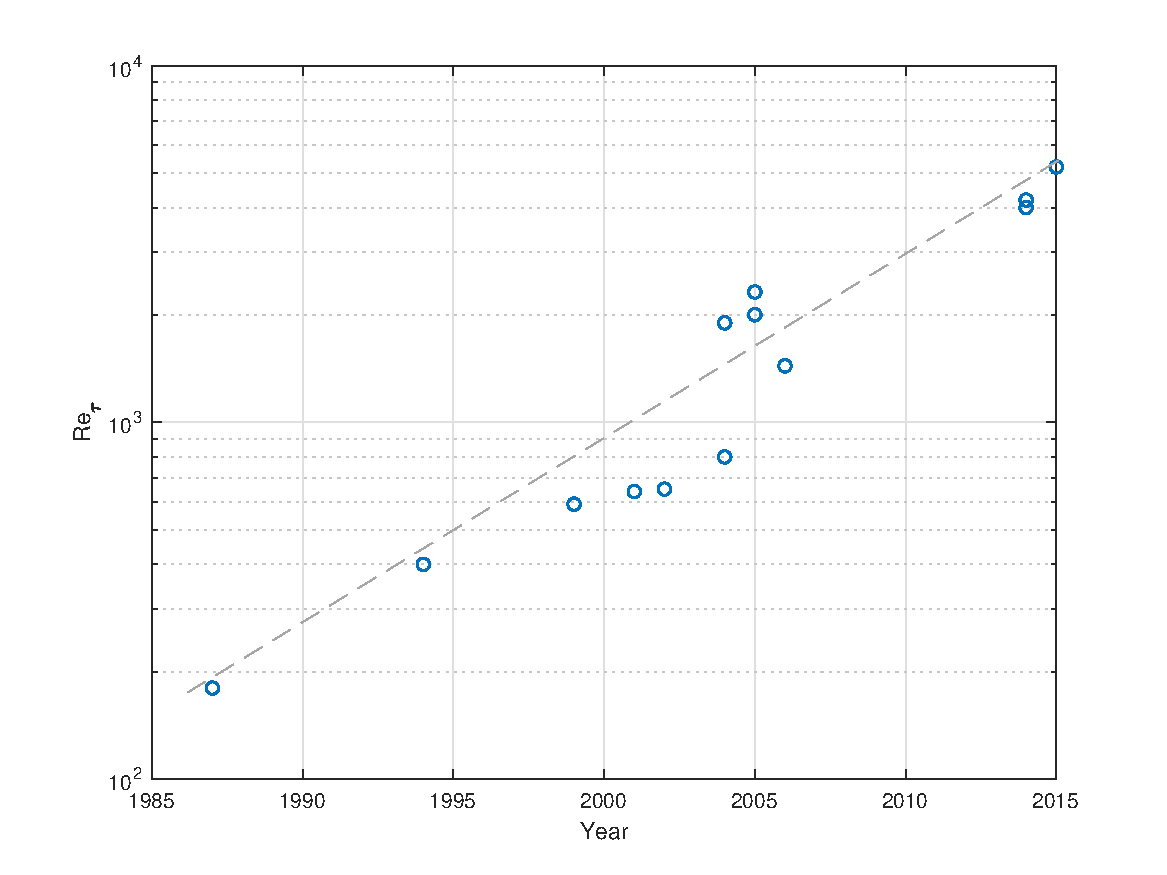
\includegraphics[width=0.8\textwidth]{grafici/dns_trend}
\caption{$Re_{\tau}$ grown trend}
\label{dns:trend}
\end{center}
\end{figure}



In this thesis our goal was to provide an highly parallelized DNS solver, based on pseudo-spectral approach, able to carry out simulation on a wide number of processors in the most efficient way possible. \par
We were particularly interested in the possibility to generate a database at very high $Re_{\tau}$ values, in reasonable time, maintaining code efficiency above the 40\%. \\~\par

In this chapter we will provide a briefly description of the phenomena, then we will recall the main statistical quantities used to characterize turbulent flows. In the second chapter we will describe the geometry of the domain along with the governing equations for the problem presented, the structure of the code, discretization, domain decomposition and I/O.
The third chapter will deal with code benchmarks while the fourth will show the results of our simulation. Finally we will draw a line of possible future works.

\section{Turbulent flows}
Every smoker can observe the nature of turbulence one inch away from their nose.
However a proper definition of turbulence is not yet given, due to the complexity of turbulence behaviour. \par
To use Prandtl words, who began an important lecture as follows: \\~\\
\emph{``What I am about to say on the phenomena of turbulent flows is still far from conclusive. It concerns, rather, the first steps in a new path which I hope will be followed by many others. The researches on the problem of turbulence which have been carried on at G\"{o}ttingen for about five years have unfortunately left the hope of thorough understanding of turbulent flow very small. The photographs and kinetographic pictures have shown us only how hopelessly complicated this flow is.''} \\~\\

Nowadays we can entrust to computational units that allows us to be no longer \emph{``hopeless''} as Prandtl was, although we are still far from having a solution, or at least a unique definition, of what the turbulence is. 
At the present time we define the turbulence as a flow regime, characterized by high Reynolds numbers and the presence of high level of diffusivity and irregularity, dissipation and three dimensional chaotic fluctuations in space and time\cite{turbulence:def}.

\section{General concepts}
An elderly definition of turbulence was provided by Hinze~\cite{Hinze}, in 1959, and say:\\~\\
\emph{``Turbulent fluid motion is an irregular condition of flow in which the various quantities show a random variation with time and space coordinates, so that statistically distinct average values can be discerned''}.\\~\\
The concept of \emph{average} is the keyword that humanity has used to start digging into the turbulence mysteries.
This kind of process, with its high sensitivity to the boundaries and initial conditions, can be defined as chaotic, so it can not be treated with a deterministic approach, therefore such randomness can be handled only by using a statistical approach.
In fact turbulence recovers its deterministic side inside statistical analysis: the detailed properties of the signal show a non predictable behaviour, but its statistical properties are consistent~\cite{Frisch}.
At statistical level, turbulent phenomena become reproducible and subject to systematic study, providing a basis for theoretical description. Therefore, the three-dimensional time-dependent Navier-Stokes equations can be solved and then the solution is averaged in order to obtain the statistics~\cite{Durbin}. 
\par
Note, however, that irregular motion and chaotic advection do not guarantee turbulence. Small point vortices can advect themselves in a chaotic manner or particles can follow complex trajectories, yet this is not turbulence. The definition, in fact, requires diffusivity. If the flow pattern looks random but does not exhibit high mix of momentum, mass and heat, it is surely not turbulent. Diffusivity is the single most important feature of turbulence, as highlighted by the experiment of Osborne Reynolds~\cite{Reynolds}, in 1883.
\par
In its famous work Reynolds has defined a ratio among inertia forces and viscous forces:
\begin{equation}
Re = \frac{ul}{\nu}
\end{equation}
\begin{figure}
\begin{center}
\includegraphics[width=1\textwidth]{grafici/reynolds_exp}
\caption{Sketch of the Reynolds experiment (\emph{left}) and flow patterns (\emph{right})}
\label{Reynolds:exp}
\end{center}
\end{figure}

with $u$ that is the characteristic velocity of the fluid, $l$ is the reference length of the scale and $\nu$ is the kinematic viscosity; able to predict the presence, or not, of the turbulence. He saw that when the inertia forces are huge the flow become unstable and the ink of its experiment started mixing with the surrounding water, as shown in the sketch of figure~\ref{Reynolds:exp}.
\par
This first work has correlated the presence of different states of the flow, laminar, transitional and turbulent, and their relationship with the couple viscous terms-nonlinear inertia term.
Further observations revealed the presence of three-dimensional eddies. Although we are still unable to determine their shapes, we have understood that they play a key role in the turbulence sustenance. Under the assumptions of incompressible flow, not subjected to external forces of volume or surface, the vorticity equation states
\begin{equation}
\frac{D \boldsymbol{\omega}}{D t} = (\boldsymbol{\omega} \cdot \boldsymbol{\nabla})\boldsymbol{u} + \nu \boldsymbol{\nabla}^{2} \boldsymbol{u}.
\end{equation}
Such equation, under a further simplification for inviscid flow, losses is rightmost term, remaining with only $ (\boldsymbol{\omega} \cdot \boldsymbol{\nabla})\boldsymbol{u}$, which determine the vortex-stretching. 
Vortex stretching is at the core of the description of the turbulence energy cascade from the large scales to the small scales in turbulence.
For incompressible flow, due to volume conservation of fluid elements, the lengthening implies thinning of the fluid elements in the directions perpendicular to the stretching direction. This reduces the length scale of the associated vorticity. Finally, at the smallest scales the turbulence kinetic energy is dissipated into heat through the action of molecular viscosity~\cite{Lumley}.


  


\subsection{Reynolds decomposition and time averaging}
The needing to employ a statistical approach require to express the quantities as a mean value plus fluctuations.\par
The expected value is calculated as a time averaged value and denoted with a bar, while the fluctuations with an appendix. Therefore we can express, for example the velocity, as
\begin{equation}
u(x,y,z,t) = \bar{u}(x,y,z) + u'(x,y,z,t).
\label{Reynolds:decomp}
\end{equation}
Two of the advantages of the Reynolds decomposition shown in equation~\ref{Reynolds:decomp} rely in the fact that the time average of the fluctuations is identically zero:
\begin{equation}
\frac{1}{T} \int_{0}^{T} u' dt =0,
\label{prop1}
\end{equation}
and the mean value is time-independent:
\begin{equation}
\frac{\partial \bar{u} }{\partial t} = 0
\label{prop2}
\end{equation}
\par
Since we have to deal with non-deterministic variables we have to define their ensemble average. In accordance with theory, an ensemble average owns a Gaussian probability distribution, thanks to the central limit theorem, so it can be no longer considered as a random variable. To be consistent with the theory we should perform $n$ times the same simulation under constant conditions.
However, in fluid dynamics, it is a common practice to exploit the ergodicity property of the processes, since, usually, the experiments are conducted under the assumption of stationary flow. 
Such property affirm that, since the process is stationary, the time averaged mean is equivalent to the ensemble average:
\begin{equation}
\langle p(\mathbf{x},t) \rangle = \frac{1}{T} \int_{0}^{T} p(\mathbf{x},t) dt.
\label{ergodic}
\end{equation}
When dealing with non-stationary processes, the equation~\ref{ergodic} is not fulfilled. Yet, this definition can still be considered valid if the sampling time $T$ is chosen small compared to the time needed for the average properties to change significantly.
\par
Expressing the Navier-Stokes equation using~\ref{Reynolds:decomp} and imposing a time averaging of the resulting equation, carrying out the simplifications due to~\ref{prop1} and~\ref{prop2}, the Reynolds averaged Navier-Stokes equation, or RANS, arise. Such equation is characterized by the appearance of a strongly non linear term, the viscous stresses term, which describe the turbulence.
\par
Although we have an equation capable of catching turbulence development using only averaged values we are still far from solving the problem. Unfortunately, the RANS equation, suffer the closure problem. We have to rely on turbulence models to evaluate the viscous, or Reynolds, stresses term. Thus we introduce an error, which is proportional to $\sqrt{u'u'}$, which is incompatible with our requirement to depict the turbulence with the highest level of fidelity possible.





\subsection{Elements of statistics}
Before introducing the concepts of correlations and spectral analysis, useful in our studies, we must define the probability density function and cumulative distribution function. \par
The cumulative distribution function is considered as the likelihood of an event to take place. It is a monotonically increasing curves and independently from its distribution it face the following properties:
\begin{equation*}
P(-\infty) = 0, \qquad P(+\infty) = 1 \qquad and \qquad \frac{\partial P(x)}{\partial x} = p(x)
\end{equation*}
where the latter term, $p(x)$, is the so called probability density function (PDF).
\par
The PDF is fundamental in the definition of the expected value
\begin{equation}
\langle u \rangle = \int_{-\infty}^{+\infty} u(x) p(x) dx
\end{equation}
and in the definition of the statistical moments
\begin{equation}
\sigma^{n} = \int_{-\infty}^{+\infty} (u(x) - \langle u \rangle)^{n} p(x)dx.
\label{statistic:momentum}
\end{equation}
Depending on the value of $n$, the equation~\ref{statistic:momentum} can define the variance ($n=2$), the skewness factor ($n=3$), the flatness factor ($n=4$) or higher statistical moments.
\par
When multiple variables are used we can recourse to the usage of the joined probability density function, $p_{x,y}(x,y)$. It exploit similar properties of the PDF and can be used to catch event characterized by the concomitancy. 
\par
It is particularly useful to determine the covariance of an event, defined as:
\begin{equation*}
\langle u_{1}u_{2} \rangle = \int_{-\infty}^{+\infty} \int_{-\infty}^{+\infty} \big( u_{1}(x_{1}) - \langle u_{1} \rangle \big) \big( u_{2}(x_{2}) - \langle u_{2} \rangle \big) p_{1,2}(x_{1},x_{2}) dx_{1} dx_{2}
\end{equation*}
\par
Starting from the result of the last equation we can define the correlation factor, $\rho_{1,2}$, as:
\begin{equation*}
\rho_{1,2} = \frac{\langle u_{1} u_{2} \rangle}{\sqrt{\langle u_{1}^{2} \rangle \langle u_{2}^{2} \rangle}}
\end{equation*}



\subsection{Correlations}

Keeping all the previous chapter definitions in mind and assuming ergodic processes, we can define the \emph{auto-covariance} factor as 
\begin{equation}
R_{uu}(\mathbf{x},\tau) = \langle u'(\mathbf{x},t) u'(\mathbf{x},t+\tau) \rangle
\label{autocovariance}
\end{equation}
The equation~\ref{autocovariance} represent the correlation between the signal from a given point in space at two different instants in time. \emph{Auto-covariance} gives an idea of the time needed by the signal itself to ``forget'' its past history, in a certain point in space. \par
The \emph{correlation coefficient} can be defined as:
\begin{equation*}
\rho(\tau) = \frac{R_{uu}(\mathbf{x},\tau)}{u_{rms}^{2}},
\end{equation*}
where $u_{rms}= \sqrt{\langle u'^{2} \rangle}$, which corresponds to $R_{uu}(\mathbf{x},0)$.\par

A similar definition could be provided to measure the correlation in space:
\begin{equation}
R_{ij}(\mathbf{x},\mathbf{r},t) = \langle u'(\mathbf{x},t) u'(\mathbf{x}+\mathbf{r},t) \rangle.
\label{covariance}
\end{equation}
The equation~\ref{covariance} represent the fluctuating parts of the velocity components correlation, set at distance $\mathbf{r}$, and it is called \emph{covariance}.\par
 



\subsection{Spectral analysis}
In the analysis of a random process, not all the necessary information can be deduced by its PDF. In the previous paragraph, correlation has proved to provide additional details about the relations established between different points in time and space. Introducing the spectral analysis enables the possibily to gain information about the energy distribution among the frequencies. In order to give a frequency description of turbulence to see which are the most energy containing frequencies, the Power Spectral Density has to be considered, and the tool used is the Fourier transform. Fourier introduced the idea to split the signal into different harmonics of different weight, in order to reproduce the signal itself. Hence, the signal domain experiences a shift, from time to frequency domain.
\begin{equation}
F(\omega) = \frac{1}{2\pi} \int_{-\infty}^{+\infty} e^{-i\omega t} f(t) dt.
\label{Fourier:t}
\end{equation}

Since the signals encountered when dealing with turbulence are continuous, a description of how the power is distributed between the different frequencies is useful. The power of a signal $u(t)$ is defined as:
\begin{equation}
P = \lim_{T \to \infty} \frac{1}{T} \int_{0}^{+\infty} u(t) dt.
\label{power:u}
\end{equation}
For numerous signals of interest, the equation~\ref{power:u} can not be casted in Fourier domain using~\ref{Fourier:t}. Therefore, the truncated Fourier transform is introduced:
\begin{equation*}
F_{T}(\omega) = \frac{1}{\sqrt{T}} \int_{0}^{+\infty} u(t) e^{i\omega t} dt.
\end{equation*}
The \emph{Power Spectral Density} can be therefore defined as:
\begin{equation*}
S_{uu} = \lim_{T\to \infty} \langle F_{T}(\omega) \rangle.
\end{equation*}
\par
One of the main interesting aspects of spectra analysis is that for a statistically stationary process, PSD constitutes the Fourier transform of the auto-covariance function $R(\mathbf{x},\tau)$:
\begin{equation*}
S_{uu} = \frac{1}{2\pi} \int_{-\infty}^{+\infty} R(\mathbf{x},\tau) e^{i\omega \tau} d\tau
\end{equation*}

and the anti Fourier transform

\begin{equation*}
R(\mathbf{x},\tau) = \int_{-\infty}^{+\infty} S_{uu} e^{i\omega t} d \omega.
\end{equation*}
\par
Since $u$ and $R(\mathbf{x},\tau)$ are both real-valued functions, their Fourier transform is an even function. Hence, $S_{uu}(\omega) = S_{uu}(-\omega)$. Here, a one-sided PSD in the positive frequency is considered
\begin{equation*}
P_{uu} = 2 S_{uu}(\omega)
\end{equation*}
If $\omega$ is positive, 0 otherwise.
\par
Frequently, it is preferred to compute the pre-multiplied one-dimensional energy spectra:
\begin{equation}
\Phi_{uu}^{+} = \frac{\alpha \Phi_{uu}}{u_{\tau}^{2}}
\label{psd}
\end{equation}
with $\Phi_{uu}$ the power spectral density of the streamwise velocity component, $\alpha$ is the streamwise wavenumber and $u_{\tau}$ the friction velocity. In this way, a more global view is allowed.
The same definition of~\ref{psd} applies also for the other two directions.




\subsection{Kolmogorov scales and viscous length scales}
In the previous sections we introduced the concept of scales. However, to completely understand the energy cascade process characteristic of turbulence, we have to define them properly.
\par
The large integral scales are the ones limited by the geometrical dimensions of the considered object. On the other hand the smallest scales are assumed to be independent of the outer geometrical restrictions and depend only on the viscosity and the viscous dissipation itself. They are referred to as the Kolmogorov scales and denoted as: length scale $\eta$, timescale $\tau_{\eta}$ and velocity scale $v_{\eta}$. 
\par
They are recovered through dimensional analysis, assuming independence among viscous dissipation $\epsilon$ and viscosity $\nu$, we can define the Kolmogorov scales as:
\begin{subequations}
\begin{align}
\eta = \sqrt[4]{ \frac{\nu^{3}}{\epsilon} }\\
\tau_{\eta} =\sqrt{ \frac{\nu}{\epsilon}}\\
u_{\eta} = \sqrt[4]{\nu \epsilon }
\end{align}
\end{subequations}

The energy cascade we talked few rows ago is the process which allows energy to transfer from the large sized scales, with their big whirls, to small scales. During such process the bigger whirls put in movement the flow, which generate smaller whirls and so on until the Kolmogorov microscales are reached. At such dimension the viscosity prevails against fluid motion, slowing it down and dissipating the energy through heat. \\~\par

Since close to the wall the main parameters of interest are the wall shear stress, $\tau_{w}$, and the kinematic viscosity, $\nu=\frac{\mu}{\rho}$, it is common practice to use values normalized on those quantities.\par
On this purpose we introduce the \emph{friction velocity} as:
\begin{equation*}
u_{\tau} = \sqrt{\frac{\tau_{w}}{\rho}},
\end{equation*}
and the \emph{viscous length scale} as:
\begin{equation*}
\delta_{\nu} = \frac{\nu}{u_{\tau}}
\end{equation*}
Combining them it is possible to define the $Re_{\tau}$ as:
\begin{equation*}
Re_{\tau} = \frac{u_{\tau}\delta_{\nu}}{\nu}
\end{equation*}
Starting from the definition of the \emph{viscous length scale} we can define the \emph{wall length scale}. \par
The \emph{wall length scale}, defined as
\begin{equation*}
y^{+} = \frac{y}{\delta_{\nu}},
\end{equation*}
is fundamental to determine the turbulence layers. Those layers divide the near wall regions, based on turbulence generation mechanism.
Starting from the wall, we find:
\begin{itemize}
\item the \emph{viscous sublayer} $(y^{+}<5)$, here the entire generation mechanism rely exclusively on viscous effects;
\item the \emph{buffer layer} $(5<y^{+}<30)$, where the turbulence generation is due to the overlapping effects of viscosity and Reynolds stresses;
\item the \emph{log-law region} $(30<y^{+}<0.1y)$, in this region we face the arise of the homonym law, that will be discussed later in detail;
\item the \emph{outer-layer} $(y^{+}>50)$, in this region the Reynolds stresses moves the turbulence engine.
\end{itemize}


  
\chapter{Problem Definition}


\section{Problem presentation}
\pagestyle{headings}

Before moving to what has been done in this thesis I wish to briefly discuss the setup of our channel flow and the equations used to solve the problem.

\begin{figure}[h]
\centering
\includegraphics[width=0.8\textwidth]{grafici/sketch_dominio}
\caption{Domain of interest}
\label{sketch_dominio}
\end{figure}

We have the domain sketched in figure~\ref{sketch_dominio} where the $x$ and $z$ coordinates denote the streamwise and spanwise directions of the flow, while the $y$ coordinate is the wall normal ones.
Along these three dimensions we have $u,v$ and $w$ components of velocity.

The flow is assumed to be periodic in the streamwise and spanwise directions. The lower wall is at position $y_l$ and the upper wall at position $y_u$. The reference length $\delta$ is taken to be one half of the channel height.
Once an appropriate reference velocity is chosen, we can define the Reynolds number as:
\[
Re = \frac{U\delta}{\nu}
\]
where $\nu$ is the kinematic viscosity of the fluid.

According to our geometry and the assumption of incompressible flow, we can express the behavior of the flow through the mass conservation law:
\begin{equation}
\frac{\partial u}{\partial x} + \frac{\partial v}{\partial y} + \frac{\partial w}{\partial z} = 0
\label{mass:cons}
\end{equation}
 and the Navier-Stokes equations, which in a dimensionless form states:
\begin{subequations}
\label{eqn:ns}
\begin{align}
\frac{\partial u}{\partial t} + u\frac{\partial u}{\partial x} + v\frac{\partial u}{\partial y} + w\frac{\partial u}{\partial z} &= 
- \frac{\partial p}{\partial x} + \frac{1}{Re} \nabla^{2}u  \label{eqn:ns:1}\\
\frac{\partial v}{\partial t} + u\frac{\partial v}{\partial x} + v\frac{\partial v}{\partial y} + w\frac{\partial v}{\partial z} &= 
- \frac{\partial p}{\partial y} + \frac{1}{Re}\nabla^{2}v \label{eqn:ns:2}\\
\frac{\partial w}{\partial t} + u\frac{\partial w}{\partial x} + v\frac{\partial w}{\partial y} + w\frac{\partial w}{\partial z} &= 
- \frac{\partial p}{\partial z} + \frac{1}{Re}\nabla^{2}w \label{eqn:ns:3}
\end{align}
\end{subequations}
The differential problem is closed when initial conditions for all the fluid variables are specified, and suitable boundary conditions are chosen. At the walls the no-slip condition are imposed.








\section{Governing equations}
The numerical method does not rely on the equations~\eqref{eqn:ns}, instead it solves the wall-normal velocity and the wall-normal vorticity equations, recovering, at the end of the the solution, the three velocity components.\\
\subsection{Wall normal vorticity equation}
Defining the wall-normal component of the vorticity vector as:
\[
\eta = \frac{\partial u}{\partial z} - \frac{\partial w}{\partial x}
\]
which, in Fourier space, holds:
\[
\hat{\eta} = i\beta \hat{u} - i \alpha \hat{w}
\] 
with the hat indicating Fourier-transformed quantities, $i$ the imaginary part, $\alpha$ and $\beta$ the streamwise and spanwise wave numbers;  allows to write a one-dimensional second-order evolutive equation for $\hat{\eta}$ which does not involve pressure, as proposed in \cite{kim_moin_moser}.

Taking the y-component of the curl of the momentum equation we obtain:
\begin{equation}
\label{curl:momentum:y}
\frac{\partial \hat{\eta}}{\partial t}  = \frac{1}{Re}  \big( D_{2}(\hat{\eta}) - k^{2} \hat{\eta} \big) + i \beta \widehat{HU} -i \alpha \widehat{HW}
\end{equation}
where $D_{2}$ is the second derivative in the wall-normal direction, $k^{2}$ is the sum of $\alpha$ and $\beta$, and the nonlinear terms are defined as:

\begin{subequations}
\label{nonlinear:terms}
\begin{align}
\widehat{HU} &= i \alpha \widehat{uu} + D_{1} \widehat{uv} + i \beta \widehat{uw}\\ 
\widehat{HV} &= i \alpha \widehat{uv} + D_{1} \widehat{vv} + i \beta \widehat{vw}\\
\widehat{HW} &= i \alpha \widehat{uw} + D_{1} \widehat{vw} + i \beta \widehat{ww}.
\end{align}
\end{subequations}

To solve the equation \eqref{curl:momentum:y} we must set suitable initial conditions for $\hat{\eta}$. Such initial conditions are computed using the initial velocity field and the definition of $\eta$ itself.
Turning such conditions into frequency domain is straightforward and satisfy the periodic boundary conditions. Finally, the \emph{no-slip} condition for velocity vector enforce the condition at the walls, which, simply, translate in $\hat{\eta}=0$ at $y=y_{l}$ and $y=y_{u}$.


\subsection{Wall normal velocity equation}
An equation for the wall-normal velocity component $\hat{v}$, which does not involve pressure, is derived in \cite{kim_moin_moser}, by summing the equation \eqref{eqn:ns:1} derived two times w.r.t. $x$ and $y$, and \eqref{eqn:ns:3} derived two times w.r.t. $y$ and $z$, then subtracting \eqref{eqn:ns:2} derived w.r.t. $x$ and $x$ and substracting once again after derivation w.r.t. $z$ and $z$.
Further simplifications are invoked through the equation \eqref{mass:cons}, which lead to the following fourth-order evolutive equation for $\hat{v}$, which is the so called wall-normal velocity equation:
\begin{multline}
\label{normal:velocity}
\frac{\partial}{\partial t} \big( D_{2}(\hat{v}) - k^{2} \hat{v} \big) = \frac{1}{Re} \big( D_{4}(\hat{v}) - 2k^{2} D_{2}(\hat{v}) + k^{4} \hat{v} \big) \\
	-k^{2} \widehat{HV} - D_{1} \big(  i \alpha \widehat{HU} + i \beta \widehat{HW} \big).
\end{multline}
To solve such equation we have to enforce initial conditions on $\hat{v}$.\\
According to Fourier expansions, the periodic boundary conditions in the homogeneous directions are automatically satisfied, whereas the no-slip condition for the velocity vector immediately translates in $\hat{v} = 0$ to be imposed at the two walls.\\
The two remaining conditions for the fourth-order equation \eqref{normal:velocity} comes from the continuity equation \eqref{mass:cons}, written at the vertical edges of the domain, $y= y_{l}$ and $y=y_{u}$.


\subsection{Velocity components in the homogeneous directions and mean flow}
As reported before, once the two preceding equations are solved, we can use them to recover the velocity components in the homogeneous directions.\par
Assuming the non-linear terms \eqref{nonlinear:terms} known, as is the case when such terms are treated explicitly in the time discretization, the equations \eqref{curl:momentum:y} and \eqref{normal:velocity} become uncoupled and, after proper time discretization, can be solved for advancing the solution by one time step, provided the nonlinear terms \eqref{nonlinear:terms} and their spatial derivatives can be calculated.
To this aim, one needs to know how to compute $\hat{u}$ and $\hat{w}$ at a given time starting with the knowledge of $\hat{v}$ and $\hat{\eta}$. \\
By using the definition \eqref{curl:momentum:y} of $\hat{\eta}$ and the continuity equation \eqref{mass:cons} written in Fourier space, a 2 $\times$ 2 algebraic system can be written for the unknowns $\hat{u}$ and $\hat{w}$; its analytical solution read:

\begin{equation}
\begin{cases}
\label{uw:eq}
\hat{u} &= \dfrac{1}{k^{2}} ( i \alpha D_{1}(\hat{v} ) - i \beta \hat{\eta})\\\\
\hat{w} &= \dfrac{1}{k^{2}} (i \alpha \hat{\eta} + i \beta D_{1}(\hat{v}))
\end{cases}
\end{equation}
For $k^{2}=0$ the system of equation \eqref{uw:eq} is singular. \par
The present method therefore enjoys its highest computational efficiency only when Fourier discretization is used in the homogeneous directions.
\par
Since the previous system of equations \eqref{uw:eq} has been obtained starting from equations \eqref{curl:momentum:y} and \eqref{normal:velocity} the solutions are sensible to homogeneous spatial derivatives through the wave numbers. \par
Let us introduce a plane-average operator defined as:
\begin{equation}
\tilde{f} = \frac{1}{L_{x}} \frac{1}{L_{z}} \int_{0}^{L_{x}} \int_{0}^{L_{z}} f \,dx \,dz.
\end{equation}
If we apply such operator to our velocity components vector $\mathbf{V}$, it turns out that $\mathbf{V}(x,y,z,t)~=~\mathbf{\widetilde{V}}(y,t) $. According to this, our velocity components are function of time and wall-normal coordinate only. In Fourier domain this behavior is denoted by the absence of the wave numbers, so for $k^{2}=0$. \par

In agreement with our reference system, where the $x$ axis is aligned with the mean flow, the temporal average of $\tilde{u}$ will denote the mean velocity profile, whereas the temporal average of $\tilde{w}=0$ throughout the channel. \\
Anyway $\tilde{w}$ can be different from zero at different time and distance from the wall. \par

Finally, applying the plane-average operator to the components of the momentum equation let us compute the $\tilde{u}$ and $\tilde{w}$:
\begin{subequations}
\begin{align}
\frac{\partial{ \tilde{u}}}{\partial t} &=  \frac{1}{Re} D_{2} ( \tilde{u}) - D_{1}( \widetilde{uv}) + f_{x} \\
\frac{\partial{ \tilde{w}}}{\partial t} &= \frac{1}{Re} D_{2}( \tilde{w}) - D_{1} ( \widetilde{vw}) + f_{z}
\end{align}
\end{subequations}

 In these expressions, $f_{x}$ and $f_{z}$ are the forcing terms needed to force the flow through the channel against the viscous resistence of the fluid. For the streamwise direction, $f_{x}$ can be an imposed mean pressure gradient, and in the simulation the flow rate through the channel will oscillate in time around its mean value. $f_{x}$ can also be a time-dependent spatially uniform pressure gradient, that has to be chosen in such a way that the flow rate remains constant in time. The same distinction applies to the spanwise forcing term $f_{z}$: in this case however the imposed mean pressure gradient or the imposed mean flow rate is zero, while the other quantity will be zero only after time average.\\
\par
\par
What has been shown in this chapter is intended just to be a brief discussion. Further informations are available in~\cite[1-3]{cpl:presentazione}.


\chapter{Code Structure}
\section{Spatial discretization along homogeneous directions}
Our solver is based on a Fourier approach. Among the advantages of such approach we face the possibility to expansion of the unknown functions in terms of truncated Fourier series in the homogeneous directions. For example the wall-normal component $v$ of the velocity vector is represented as:
\begin{equation}
v(x,y,z,t) = \sum_{h=-nx/2}^{+nx/2} \sum_{l=-nz/2}^{+nz/2} \hat{v}_{hl}(y,t) e^{i\alpha x}e^{i \beta z}
\end{equation}
where:
\begin{equation}
\alpha = \frac{2\pi h}{L_{x}} = \alpha_{0} h; \quad \beta= \frac{2 \pi l}{L_{z}} = \beta_{0}l
\end{equation}

$h$ and $l$ are integer indexes corresponding to the streamwise and spanwise direction respectively, and $\alpha_{0}$ and $\beta_{0}$ are the fundamental wavenumbers in these directions, defined in terms of the streamwise and spanwise lengths $L_{x} = {2\pi}/{\alpha_{0}} $ and $L_{z} = {2 \pi}/{\beta_{0}}$ of the computational domain. The computational parameters given by the streamwise and spanwise lenght of the computational domain, $L_{x}$ and $L_{z}$ , and the truncation of the series, $nx$ and $nz$, must be chosen so as to miminize computational errors. For further details regarding the proper choice of a value of $L_{x}$ see~\cite{QuadrioMaurizio2003Issi}.

The convolutions required to solve the equations~\ref{curl:momentum:y} and~\ref{normal:velocity} are computationally expensive if carried out in the frequency domain. The same evaluation can be performed efficiently by first transforming the three Fourier components of velocity back in physical space, multiplying them in all six possible pair combinations and eventually retransforming the results into the Fourier space. Fast Fourier Transform algorithms are used to move from Fourier to physical space and viceversa. The aliasing error is removed by expanding the number of modes by a factor of at least $3/2$ before the inverse Fourier transforms, to avoid the introduction of spurious energy from the high-frequency into the low-frequency modes during the calculation.



\section{Finite difference scheme}


\subsection{Compute of the finite difference coefficients}




\section{Time Discretization}





\section{Domain Decompositions}
The engine of Quadrio and Luchini described into~\cite{cpl:presentazione} works per \emph{y-slabs}, as shown in figure~\ref{domain_decomp},
\begin{figure}
\centering
\includegraphics[width=0.8\textwidth]{grafici/decomp_dominio_cpl}
\caption{Original domain decomposition in case of 4 processors}
\label{domain_decomp}
\end{figure}
 allowing to perform convolutions and Fourier transformations locally on each processor, avoiding the cost of non-local transposition for the velocity array and the non-linear terms ones. Such implementation, denominated pipelined-linear-system (PLS), lead to a minimum of communication, in fact this approach require to send and receive only the values stored in the two upper and lower boundary cells of the local decomposition, in order to provide the data required by the fourth-order finite difference scheme.
 \par
 Using the PLS approach the number of bytes exchanged in a three step Range-Kutta method are:
 \begin{equation}
 D_{t} = 3 \times 8 \times (p-1) \frac{3}{2} \times \frac{nx}{p} \frac{nz}{p} \times ny \times 18
 \label{exchange:data:cpl}
 \end{equation}
 where:
 \begin{description}
  \item[3] takes into account the number of time steps;
  \item[8] for counting the bytes;
  \item[$\mathbf{(p-1)}$] is the number of nodes across which the exchange take place;
  \item[ $\mathbf{\frac{3}{2}}$ ] corresponds to the expansion in horizontal modes required by the dealiasing process;
  \item[ $\mathbf{\frac{nx}{p} \times \frac{nz}{p}}$] is the grid portion, for each plane, to exchange with the others nodes;
  \item[18] due to the 3 velocities plus the 6 products to be exchanged twice, before and after the FFT;
  \item[ny] takes into account the number of planes to be exchanged.
\end{description}
Further details about the PLS communications are available in \cite[\nopp chapter 4.2]{ns:quadrio}. \\
 \par
Although efficient for small processors grid, the performances of this approach falls quickly whether the processors number becomes comparable with \emph{ny}.  Furthermore the code structure limit the number of parallel process to be just a fraction of the \emph{ny} extension.
\par
To avoid such limitations and increase the number of parallel processes we decided to move from PLS approach to something different.
We have identified two possible solutions:
\begin{description}
  \item employ \textbf{slab} decomposition along x or z axis;
  \item employ \textbf{pencil} decomposition.
\end{description}
Both implementation require extensive use of the MPI paradigm and, possibly, a library to handle such decompositions.
We opted to employ OpenMPI\cite{openmpi} for what concern the MPI paradigm, in particular we entrust to the well established OpenMPI version 3.1, release 3.1.3.
The ideas behind the choice of such library rely on the fact the OpenMPI is released behind BSD license\cite{bsd:license}, it is designed to group different MPI implementation, avoiding fragmentation and forking problem\cite{faq:openmpi} and, although less optimized on proprietary fabric such as Intel Omni-Path fabric\cite{intel:omnipath}\cite{intel:intelmpivsopenmpi}, is wider spread.


 while, for the decomposition, we entrusted in a new library, released by the 


\subsection{Slabs decomposition}


\subsection{Pencil decomposition}


%\section{Parallel I/O}

Input-output could be a serious bottleneck if we do not pay the right attention.
In particular, when dealing with supercomputers, two major problems arise:
\begin{itemize}
\item needing of parallel I/O,
\item avoid endianness problem related.
\end{itemize}
As first thing let us introduce I/O.\par
\begin{wrapfloat}{figure}{l}{0pt}
\includegraphics[width=0.5\textwidth]{grafici/masterslave}
\caption{Master-Slaves I/O setup}
\end{wrapfloat}
In computer architecture, the combination of the CPU and main memory, to which the CPU can read or write directly using individual instructions, is considered the brain of a computer. Any transfer of information to or from the CPU/memory combo, for example by reading data from a disk drive, is considered I/O~\cite{io}.
When dealing with cluster the transit of data from disk to CPU is not so straightforward. The presence of multiple CPU require the adoption of one of the following strategies.\par
The most basic strategy is the master-slaves setup. In this kind of strategy a single node of the grid have access to the storage, therefore no scalability is provided. The slave nodes must send/receive data from the master, therefore we face strong slowdown related to the huge workload required to perform I/O by the single node and the following communications among nodes.\par
A second approach is shown here beside and consist in performing distributed I/O on local files. Such kind of implementation is scalable, ensure data consistency and avoid communication during I/O phase. 
\begin{wrapfloat}{figure}{r}{0pt}
\includegraphics[width=0.5\textwidth]{grafici/localio}
\caption{Distributed I/O on local files}
\end{wrapfloat}However, since every processor writes data on its own hard storage, it require a great deal of post processing work to glue data among each others, which increase linearly with the number of processes. For this reason we can not consider it affordable. \\
\begin{wrapfloat}{figure}{r}{0pt}
\includegraphics[width=0.5\textwidth]{grafici/mpiio}
\caption{Coordinated controlled accesses}
\end{wrapfloat}
\par
The last kind of I/O setup, which is the most updated and optimized, is the so called coordinated controlled accesses.
Scalability reaches its peak with this kind of implementation, which takes care of possible communications needing by its own.
In this approach every CPU can access to the single storage memory in which the dataset is hosted, and in concomitancy with the other processes, writes the data. As can be understood, the reading/writing operation is intrinsically fragile, since guarantee data consistency can be hard. To avoid consistency lacks, the MPI-IO has been introduced with the deployment of MPI-2 standard~\cite{MPI:standard2}.

On top of MPI-IO several high level I/O libraries arose, two well established examples are parallel netCDF and parallel HDF5. 

At exception of the master-slave approach, every presented strategy require the adoption of a parallel file system.
In computing, a file system or filesystem controls how data is stored and retrieved. Without a file system, information placed in a storage medium would be one large body of data with no way to tell where one piece of information stops and the next begins. By separating the data into pieces and giving each piece a name, the information is easily isolated and identified. We can briefly define the file system as the structure and logic rules used to manage the groups of information and their names.
In the same fashion a parallel file system maintains logical space and provides efficient access to data for distributed memory configurations.\\
\par
Let us establish the concept of endianness.
Intel introduces their white paper with the following sentence:\par
``Endianness describes how multi-byte data is represented by a computer system and is dictated by the CPU architecture of the system. Unfortunately not all computer systems are designed with the same Endian-architecture. The difference in Endian-architecture is an issue when software or data is shared between computer systems''\cite{endianness}.\par
Since our binary database has been built on Marconi, at Cineca, but the post-processing analysis take place on our personal computers, we need to guarantee results portability with a reliable method to store the data. \\
\par
Unfortunately MPI-IO can not set a bit ordering different from the machine's natives ones, and we can not assure portability in this way. To do so we have to move from MPI-IO to a library capable to satisfy our requirements.\par
Employ the well established parallel HDF5 library is the natural choice.





\chapter{Code Benchmarks}
\section{Scaling Performance of $128^3$ problem}
\pagestyle{headings}


\section{Scaling Performance of $256^{3}$ problem}
The medium sized problem shows better scaling performances compared to the small ones.
This behavior, in which bigger problems provide better scaling capabilities, has been highlighted and discussed by many authors in past.
After a little preamble about scaling let us dig into results.\\
\par
A slab decomposed algorithm provide gains of $\mathcal{O}(10)$ in terms of execution times, less than a pencil decomposed algorithm, but with better results for small processors grid. In fact, as depicted in figure~\ref{1281} the 1D decomposition curve achieve lower execution times than the 2D ones, until 8 cores.\\
Passed 8 cores the pencil decomposition prevails, reaching speedup factors above 100, with time savings in the order of magnitude of $\mathcal{O}(100)$ with respect to the single core runtime.
In the figure~\ref{1283} is possible to see the efficiencies achieved by the two methods, running on 64 threads per processor. It is important to denote the behavior of the pencil decomposed algorithm, which, until 8 cores in use, exhibits high scaling efficiency.
Passed 8 cores, to recover high efficiency we must decrease the number of threads per processor.
\section{Scaling Performance of $512^3$ problem}
Let us proceed now showing the performances achieved by our code in a medium sized problem.
The present simulation shown a better scaling effectiveness and efficiency for both methods with respect to $128^{3}$ problem. 
\par
Once again the best results are reached using 64 cores per processor, possibly indicating that the array dimension fits in the cache memory.
\par
The speedup peak is remarkable, with a factor of $260$ on $2048$ cores using pencil decomposition, while stops around $38$ using $128$ cores and slab decomposition. \\
\par

\begin{figure}
\begin{center}
\includegraphics[scale=0.6]{grafici/5121}
\caption{Scaling performance of $512^3$ simulation}
\label{5121}
\end{center}
\end{figure}

\begin{figure}
\begin{center}
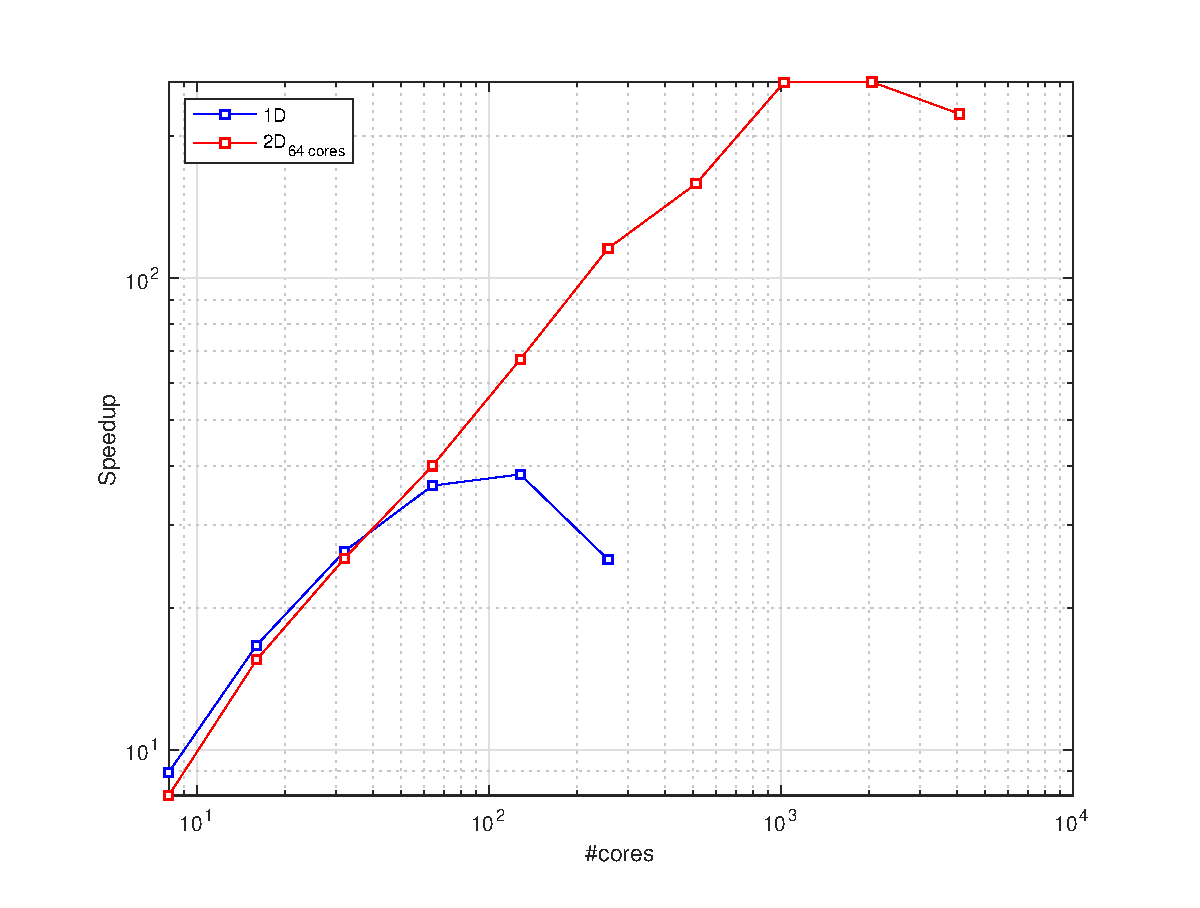
\includegraphics[scale=0.6]{grafici/5122}
\caption{Speedup performance factor of $512^3$ simulation}
\label{5122}
\end{center}
\end{figure}

As we can see from figure~\ref{5122}, the speedup factor of the 2D decomposed algorithm increase approximately linearly until $256$ cores. The raise in performance continue at lower factor until $1024$ cores are reached, where nearly stops before start descending once passed $2048$ cores.
The inverse behavior is shown in figure~\ref{5121}, where the simulation time is plotted against the number of cores.\\
In figure~\ref{5121} is also reported the theoretical scaling limit. Comparing this line, in dashed green, with our results let us conclude that our scaling, although linear for the majority of the time, is sub-optimal. 
The same reasoning is valid also for the slab decomposed algorithm, although in a smaller region of cores number.
It is interesting to denote the advantageous behavior of such algorithm until $64$ cores, where both performances are still slightly different in terms of speedup factor. 
\par
By looking at the values in table~\ref{512data} of page~\pageref{512data} and the depicted counter part, in figures~\ref{5121} and \ref{5122}, it is possible to denote that between $8$ and $16$ cores the loss are really small. This lead us to expect a perfect theoretical linear behavior from $1$ to $16$ cores. Keeping this in mind, we feel confident and seems reasonable to consider a speedup factor of $8$ for the $8$ cores simulation, possibly doing an error below the unit. \\
\par
We refer to figure~\ref{5123} to have an idea of the efficiency of the algorithm. The figure shows that the efficiency remains above $80\%$ until $32$ cores are used. However, once passed such limit, the behavior is linear and smoother with respect to the ones shown in figure~\ref{644} of page~\pageref{644}.

\begin{figure}
\begin{center}
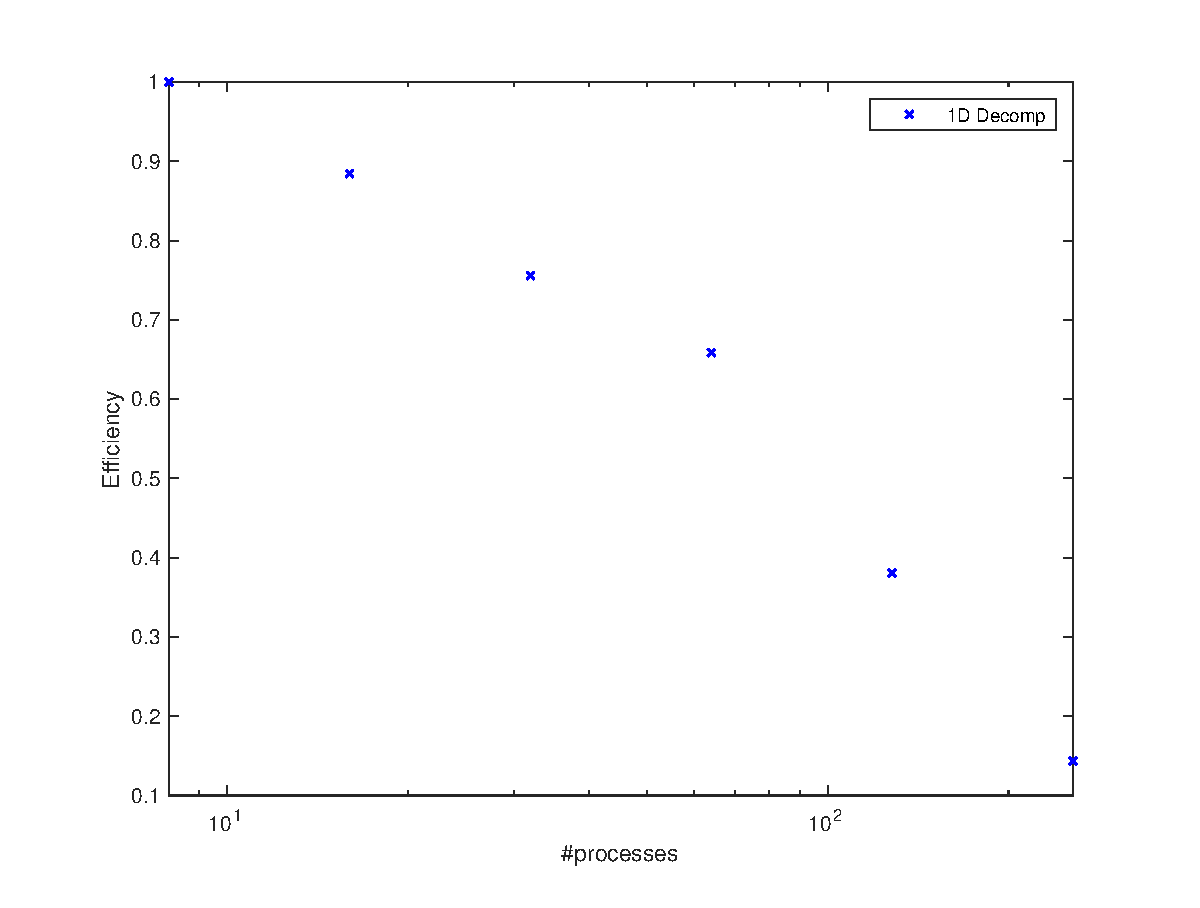
\includegraphics[scale=0.6]{grafici/5123}
\caption{Efficiency factor of $512^3$ simulation}
\label{5123}
\end{center}
\end{figure}


\begin{table}[h]
\caption{Data from $512^{3}$ simulation, if present first row indicates 1D decomposition}
\begin{center}
\begin{tabular}{c c c c}
\toprule
\textbf{\#cores} & \textbf{Time [s]} & \textbf{Speedup} & \textbf{Efficiency [\%]} \\
\midrule
\multirow{2}{*}{8} & 1750 & 8.96 & 112 \\
& 1960 & 1 & 100 \\
\hline
\multirow{2}{*}{16} & 941.5 & 16.65 & 104 \\
& 1011 & 15.51 & 97 \\
\hline
\multirow{2}{*}{32} & 595.3 & 26.35 & 82 \\
& 616.2 & 25.45 & 80 \\
\hline
\multirow{2}{*}{64} & 432.1 & 36.3 & 57 \\
& 392.3 & 39.97 & 62 \\
\hline
\multirow{2}{*}{128} & 409.2 & 38.34 & 30 \\
& 233.2 & 67.22 & 53 \\
\hline
\multirow{2}{*}{256} & 620.1 & 25.29 & 10 \\
& 135.7 & 115.5 & 45 \\
\hline
512 & 99 & 158.4 & 31 \\
1024 & 60.4 & 259.6 & 25 \\

\bottomrule
\end{tabular}
\end{center}
\label{512data}
\end{table}%
\section{Scaling Performance of $4096\times512\times256$ problem}
The last benchmark deal with very large problems. Like for the previous large problem, the dimensions are so huge to require the adoption of multiple processors to run, otherwise we will face an out of memory error.
On a Intel Xeon Phi~\cite{intel:xeonphi} the minimum requirements are to employ at least 2 processors and use 32 cores, or less, per processor.
\par
As the previous problem have highlighted, the less cores are used and the better results are scored, so our impossibility to go further than 32 cores per processor, as pointed some rows before, would not be a big deal. We may suppose that the poorest results will be achieved by 32 cores runs, instead of the 64 ones. \\
\par

\begin{figure}
\begin{center}
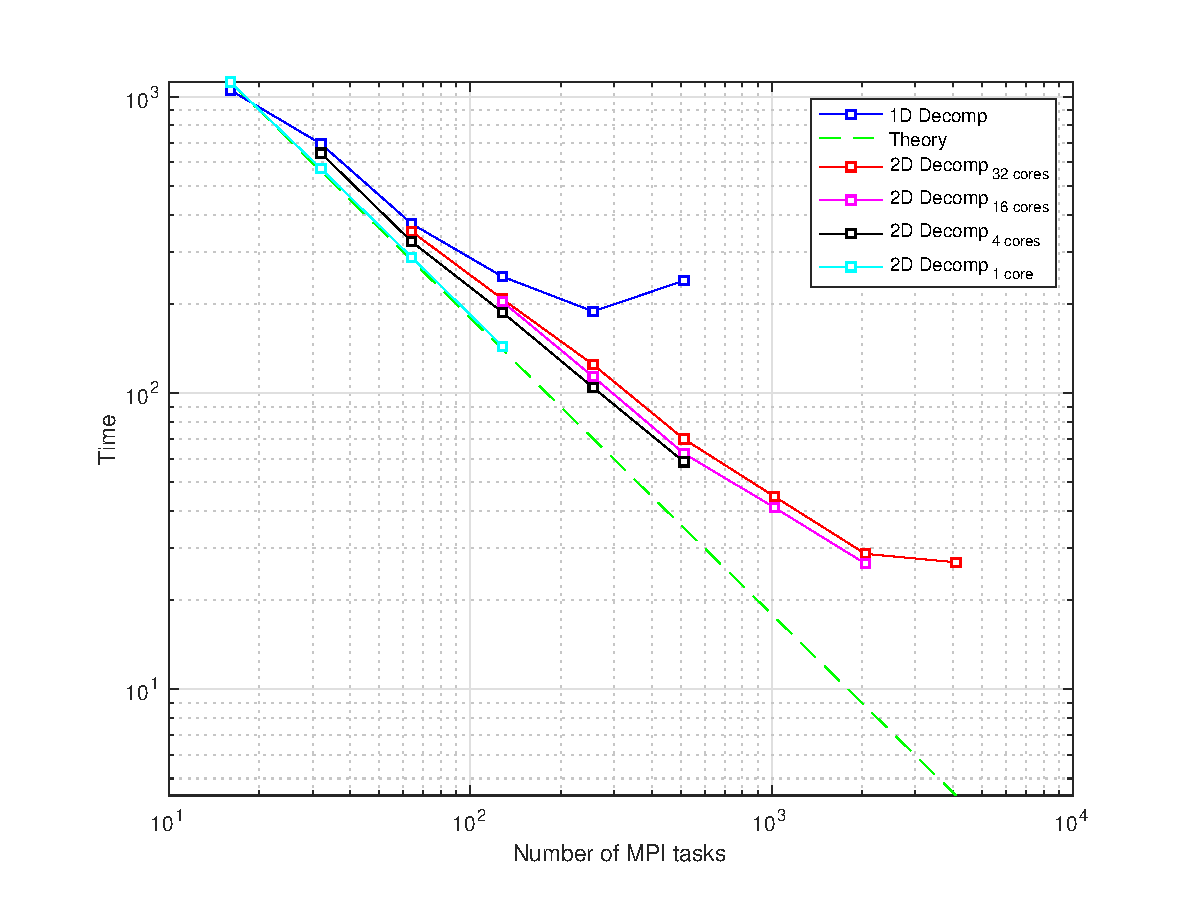
\includegraphics[scale=0.6]{grafici/20481}
\caption{Time scaling comparison for $4096\times 512\times 256$ simulation}
\label{20481}
\end{center} 
\end{figure}

Let us start showing figure~\ref{20481} in which is reported the time scaling of our code.\par
As could be seen, the 2D decomposition using single core achieved the lowest timing execution.
It is interesting to denote how this combination fits the theoretical behavior perfectly.\par
All other 2D decomposed combinations exploit a worse behavior with respect to the single core run, with a marked trend, where the increase in cores per processor number leads to poorer performances. \par 
Such behavior is aligned with our predictions.\\

\begin{figure}
\begin{center}
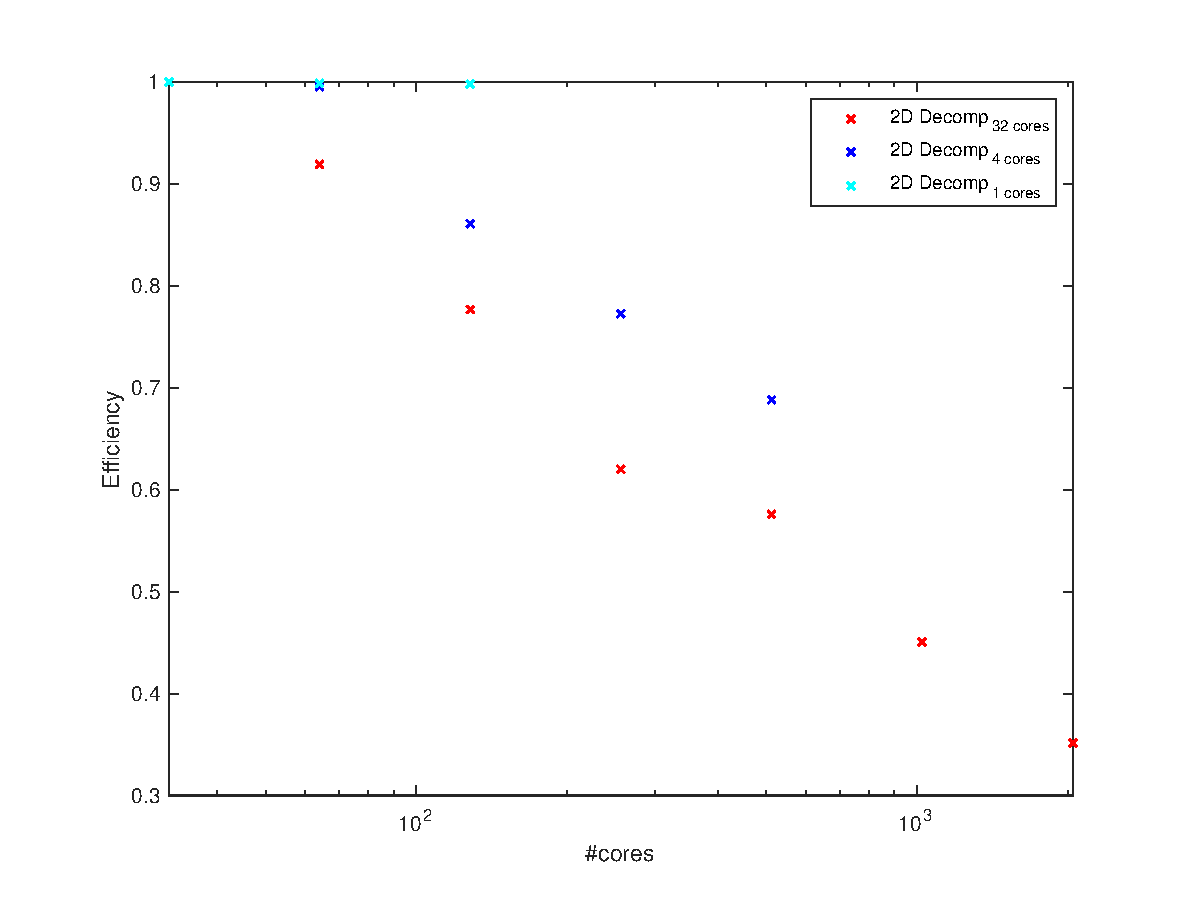
\includegraphics[scale=0.6]{grafici/20483}
\caption{Efficiency factor of $4096\times512 \times256$ simulation using 1D decomposition}
\label{20483}
\end{center}
\end{figure}

\begin{table}
\caption{Data from $4096\times 512\times 256$ simulation, 1D decomposition}
\begin{center}
\begin{tabular}{c c c c}
\toprule
\textbf{\#Processes} & \textbf{Time [s]} & \textbf{Speedup} & \textbf{Efficiency [\%]}\\
\midrule
16 & 1052.9 & 16 & 100\\
32 & 693 & 24.31 & 76\\
64 & 372.5 & 45.23 & 71\\
128 & 247 & 68.2 & 53\\
256 & 188.5 & 89.37 & 35\\
512 & 239.5 & 70.34 & 14\\
\bottomrule
\end{tabular}
\end{center}
\label{2048:data:1}
\end{table}

\par
For what concern about the 1D decomposed algorithm, which, since the code structure is slightly different, can run also on 64 cores per processor, it achieve the worst performances among all possible solutions, highlighting once again the benefits of using a pencil decomposed approach. \par
The speedups achieved by this kind of domain decomposition can be seen in table~\ref{2048:data:1}, on page~\pageref{2048:data:1}, while the efficiency graph, which shows a poor behavior, can be seen in figure~\ref{20483}. \\
\par



Far more interesting, are the data in table~\ref{2048:data:2}, which report the speedups, efficiency and timing achieved by the algorithm with 2D decomposition. The data, and the graphical counterpart which can be seen on page~\pageref{20482} in figure~\ref{20482} and~\ref{20484}, report a very high efficiency using single core, while, although smaller, a still high efficiency is preserved by using 4 cores per processor.\\
\par
\begin{figure}
\begin{center}
\includegraphics[scale=0.6]{grafici/20484}
\caption{Efficiency factor of $4096\times512 \times256$ simulation using 2D decomposition}
\label{20484}
\end{center}
\end{figure}
Increasing the counter of threads per processor leads to constant losses, as expectable. However, such losses between adjacent stations are lower than the ones of the previous simulations, furthermore we can see wider gaps among the efficiency curves, symptom that there is wider room for improvements.\par
Moreover, at very high number of cores, the efficiency curves slope is minor than before, preserving efficiency and allowing us to perform faster computations with greater speedups.\\
\par
To talk about speedups is useful to introduce figure~\ref{20482}, in which these are reported.\par
The graph, on page~\pageref{20482}, shows the results achieved by the 1D and 2D domain decomposed algorithm, with emphasis on the effects of the variation of cores per processor quantity, for the 2D algorithm only.\par
As has been done in the previous section, the high efficiency shown by the single core run, combined with the physical impossibility to use less cores, has lead us to made the assumption of speedup equal to 16 for a 16 parallel processes run in a single core environment.All other efficiencies and speedups have been derived using such data as reference.\\
\par

\begin{table}
\caption{Data from $4096\times 512\times 256$ simulation, 2D decomposition}
\begin{center}
\begin{tabular}{c c c c c}
\toprule
\textbf{\#Processes} & \textbf{Time [s]} & \textbf{Speedup} & \textbf{Efficiency [\%]} & \textbf{cores}\\
\midrule
16 & 1121.5 & 16 & 100 & 1\\
\hline
\multirow{2}{*}{32} & 571.4 & 31.4 & 98 & 1\\
& 644.8 & 27.83 & 87 & 4\\
\hline
\multirow{3}{*}{64} & 287.2 & 62.47 & 98 & 1\\
& 323.9 & 55.39 & 87 & 4\\
& 350.7 & 51.17 & 80 & 16\\
\multirow{4}{*}{128} & 143.8 & 124.8 & 98 & 1\\
& 187.2 & 95.85 & 75 & 4\\
& 203.4 & 88.23 & 69 & 16\\
& 207.5 & 86.47 & 68 & 32\\
\hline
\multirow{3}{*}{256} & 104.3 & 172 & 67 & 4\\
& 113.4 & 158.2 & 62 & 16\\
& 124.6 & 144 & 56 & 32\\
\hline
\multirow{3}{*}{512} & 58.6 & 306.4 & 60 & 4\\
& 62.5 & 287.1 & 56 & 16\\
& 70 & 256.5 & 50 & 32\\
\hline
\multirow{2}{*}{1024} & 41 & 437.5 & 43 & 16\\
& 44.7 & 401.4 & 39 & 32\\
\multirow{2}{*}{2048} & 26.6 & 675.5 & 33 & 16\\
& 28.7 & 626.3 & 31 & 32\\
\hline
4096 & 26.8 & 668.8 & 16 & 32\\
\bottomrule
\end{tabular}
\end{center}
\label{2048:data:2}
\end{table}

As can be seen in table~\ref{2048:data:2} the best result is achieved using 16 cores per processor and 2048 parallel processes. Unfortunately, due to some policy limitations, we can not push forward our resources request, although the graph clearly shows margins of improvements for such configuration.\\
\par
Differently from all the previous simulations, the processor grid for the pencil decomposition results balanced when the streamwise stencil has half the modes with respect to the other direction. Such configuration has been suggested by benchmarks.
\par
In conclusion we may say that, although the modes distribution results unbalanced in this simulation, the speedup trend still remain aligned with the ones exhibited in the other simulations.
\begin{figure}
\begin{center}
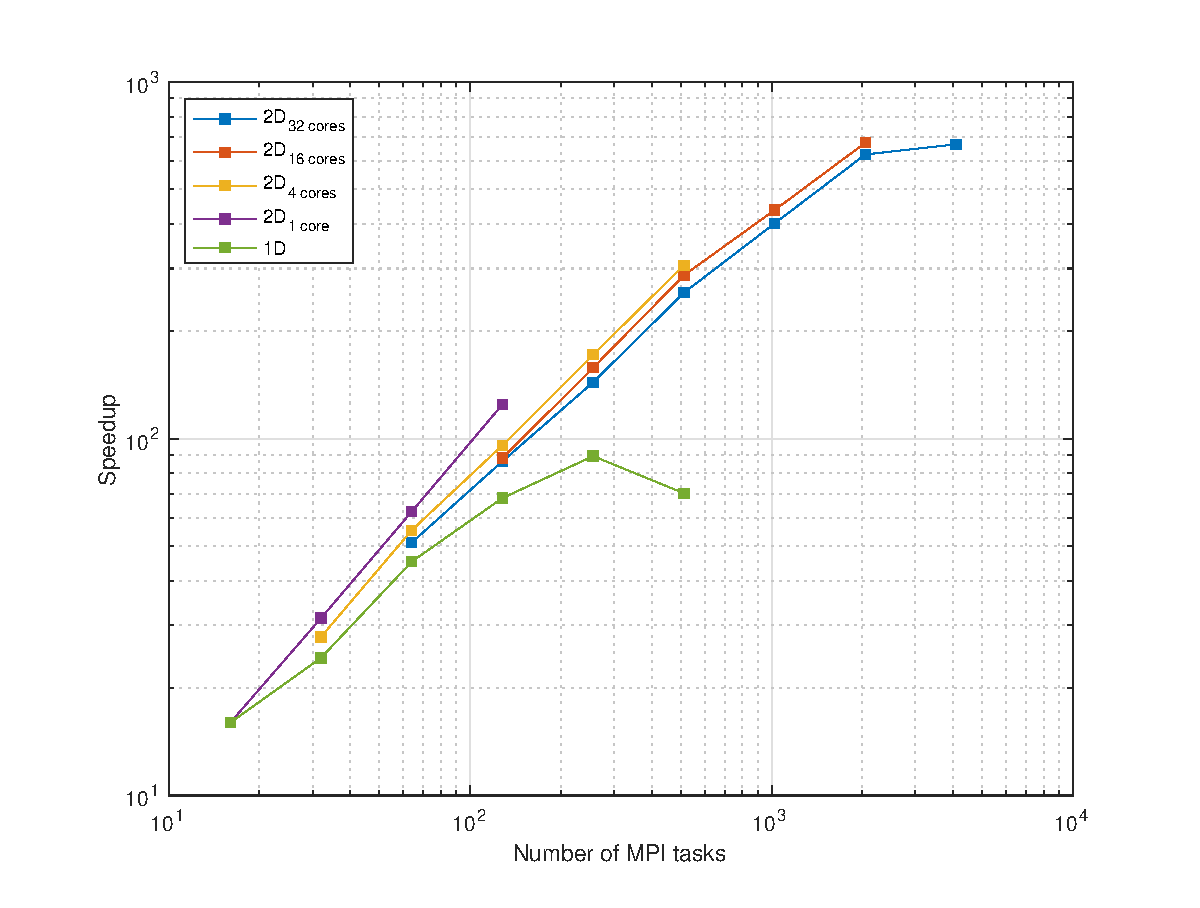
\includegraphics[scale=0.6]{grafici/20482}
\caption{Speedup factor of $4096\times512 \times256$ simulation}
\label{20482}
\end{center}
\end{figure}





\section{Benchmarks conclusions}
The benchmark series has highlighted common trends present in our simulations.
\par
By looking at the curves, we can see that the performances envelope is bordered by the 64 cores run and the single core ones.  We can catch from the graphs that the code tends to perform faster using as less threads per processor as possible.  This behavior is reasonable, since our code and the library in which we rely on to perform the MPI transposition, does not implement the OpenMP technology at the moment, so, although we could carry on the simulation basing our communications on MPI, we will experience efficiency lacks when dealing with intra-node messagings. In particular, when dealing with many cores per processor we face a speedup tendency to pass from 2 to $2^{2/3}$, as the number of MPI tasks gets doubled, as highlighted in~\cite{dns:gpu:supercomputer}. \par
Unfortunately, the Intel KNL's architecture~\cite{intel:xeonphi} is designed to exploit code vectorization as much as possible and OpenMP plays a key role in this kind of implementations. \par
We suggest to move to traditional processors architectures, instead of using MIC, to experience lower losses. Our simulations in fact has highlighted that, although MPI can not guarantee high efficiency in heavily threaded applications, the lacks using 16 cores, or less, per processor can be acceptable.\\
\par
As the problem size grows, the optimal number of MPI tasks, to achieve the best speedup, grows. In fact, we passed from 512 parallel processes for a $128^{3}$ simulation to 2048 for a $512^{3}$ simulation. \par

\begin{figure}
\begin{center}
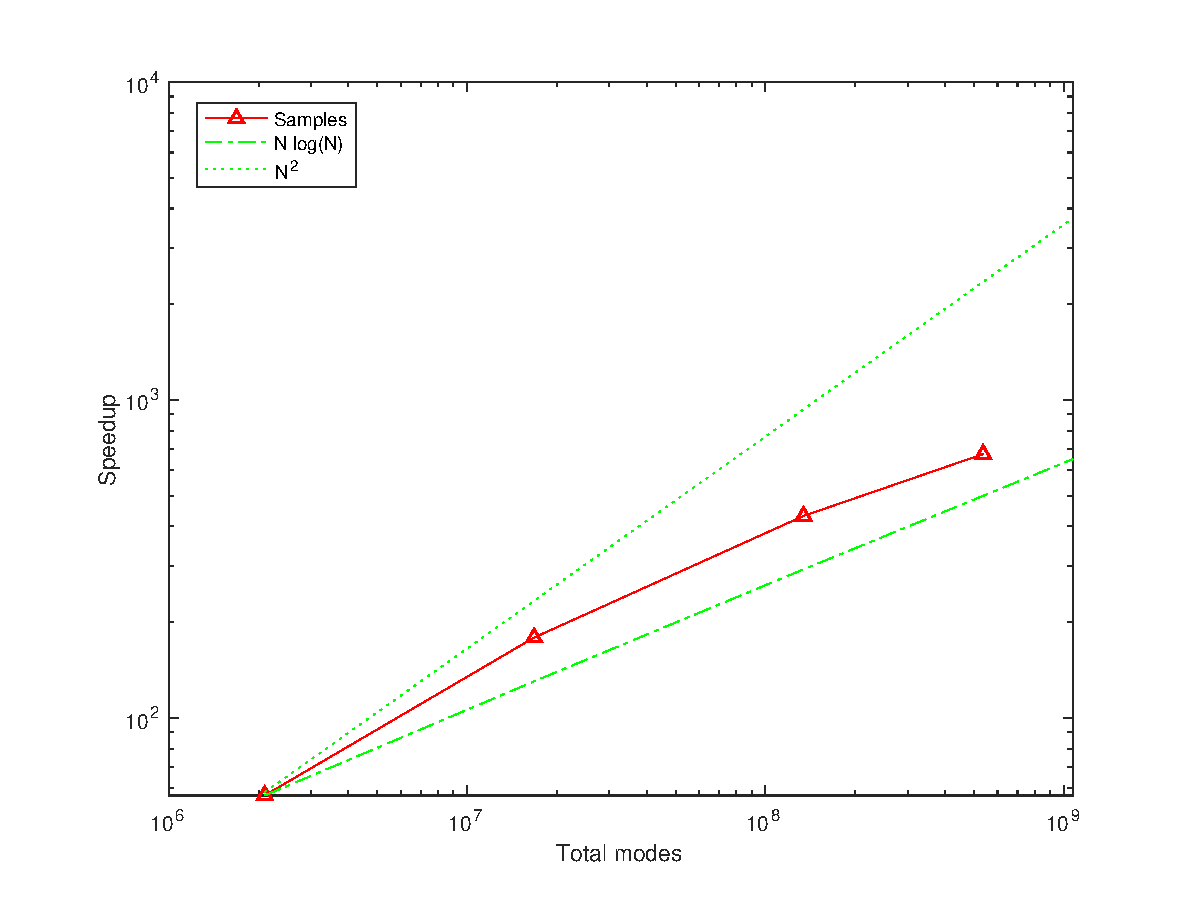
\includegraphics[scale=0.6]{grafici/speedup_trend}
\caption{Speedup factors growth}
\label{speedup:trend}
\end{center}
\end{figure}

On the other hand, the speedup factor increase its peak in a fashion which lies between $N\log(N)$ and $N^{2}$, like testify by figure~\ref{speedup:trend} in which our samples are plotted against such behaviors. \\
\par

Let us introduce the speedup comparison with hyper threading turned on. \par
Hyper threading is a technology developed by Intel~\cite{hyper:paper}  that virtually doubles the cores on the CPU, making the CPU run faster and more efficient by scheduling the workload between the cores. On modern Xeon Phi we can quadruplicate the number of cores, obtaining until 272 threads per processor. However, as our benchmark shows, this technology does not provide a boost in terms of speedup, on the contrary it penalizes our results in evident fashion.\par
In figure~\ref{hyper} are compared the original results of a $512^{3}$ simulation, running on different cores per processor, against two curves which exploit the hyper threading technology.\\
\par
In conclusion we would like to show the cost for a single degree of freedom (DOF) in terms of CPU time.
Such cost has been obtained considering the simulation time, the number of time steps required by the simulation and the total number of degrees of freedom, so it has to be intended as a mean value.
The cost is defined as:
\begin{equation}
Time/DOF = \frac{Sim Time}{timestep}\times \frac{1}{nx\times ny\times nz}
\end{equation}
Our results have been compared with the ones achieved in~\cite{Borrel}, where a boundary layer simulation is carried out on a flat plate, through direct numerical simulation, on JUGENE, a Blue Gene P architecture~\cite{blue:gene:chip}\cite{blue:gene:network} installed at Juelich Forschungszentrum, with its 32,768 cores.\par
Since the problems compared are just similar we can only obtain qualitative informations from that.

\begin{figure}
\begin{center}
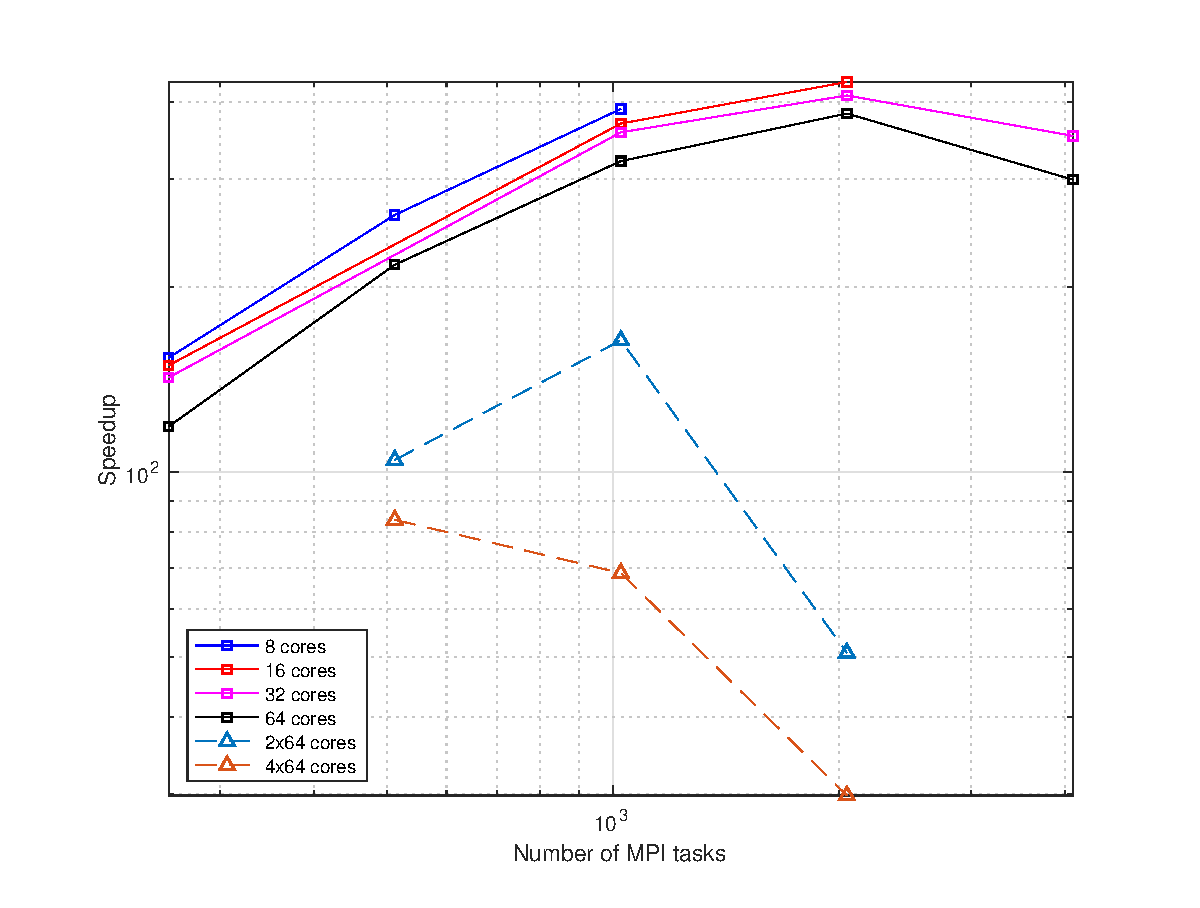
\includegraphics[scale=0.6]{grafici/hyperthreading}
\caption{Hyper threading benchmark}
\label{hyper}
\end{center}
\end{figure}

\begin{figure}
\begin{center}
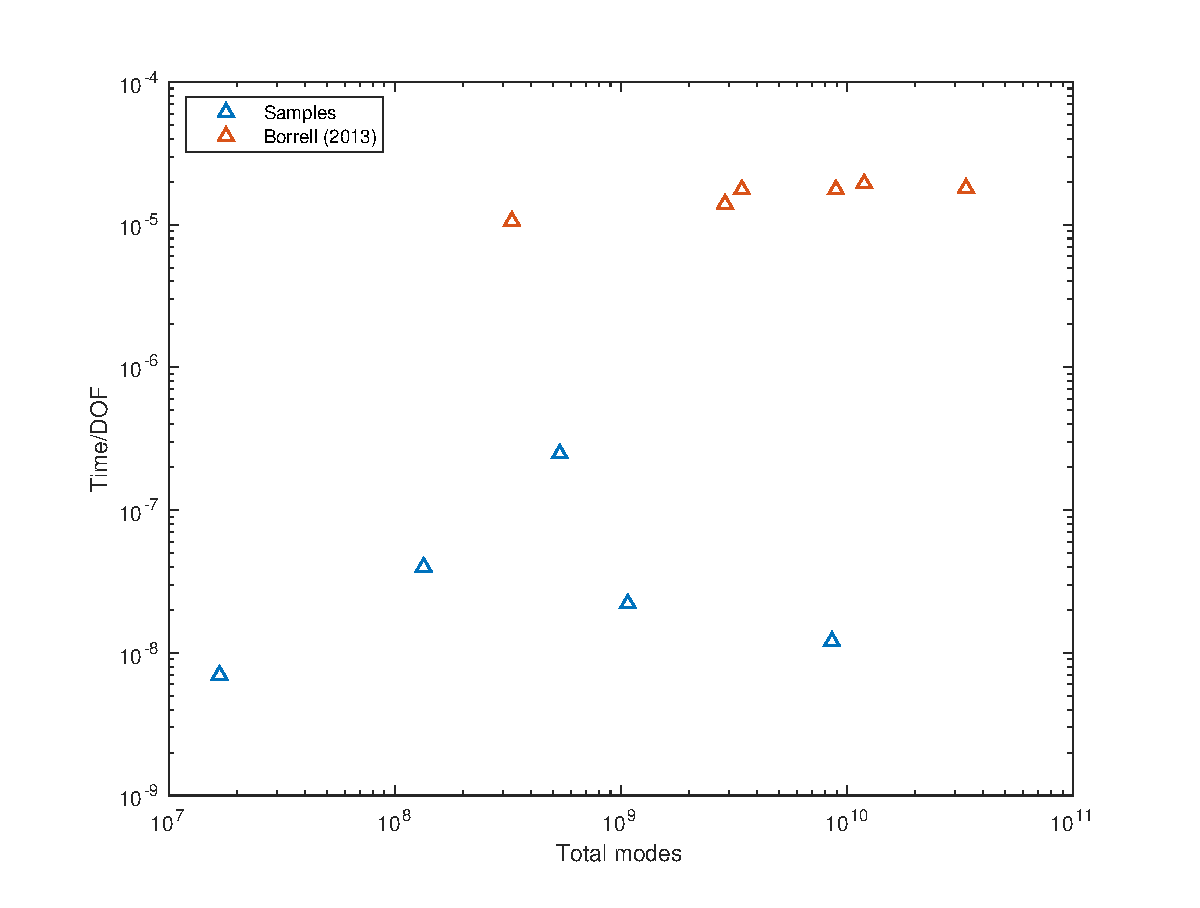
\includegraphics[scale=0.6]{grafici/time_dof}
\caption{Qualitative comparison of Time-DOF ratio}
\label{hyper}
\end{center}
\end{figure}

\chapter{Simulations results}
\section{$\mathbf{Re_{\tau}=180}$ simulation}

The $Re_{\tau}=180$ simulation has been used to validate our results against the~\cite{kim_moin_moser} ones. \par
The graphs~\ref{loglaw_180} and~\ref{budget_180} show the behavior of the $\bar{u}^{+}$ and the TKE budgets in the near wall region, with $\bar{u}^{+}$ indicating the mean velocity profile, adimensionalized using friction velocity. \par
In both figures we reported the \emph{Kim et al.} results, using dotted line, for comparison. \\~\par

\begin{figure}
\begin{center}
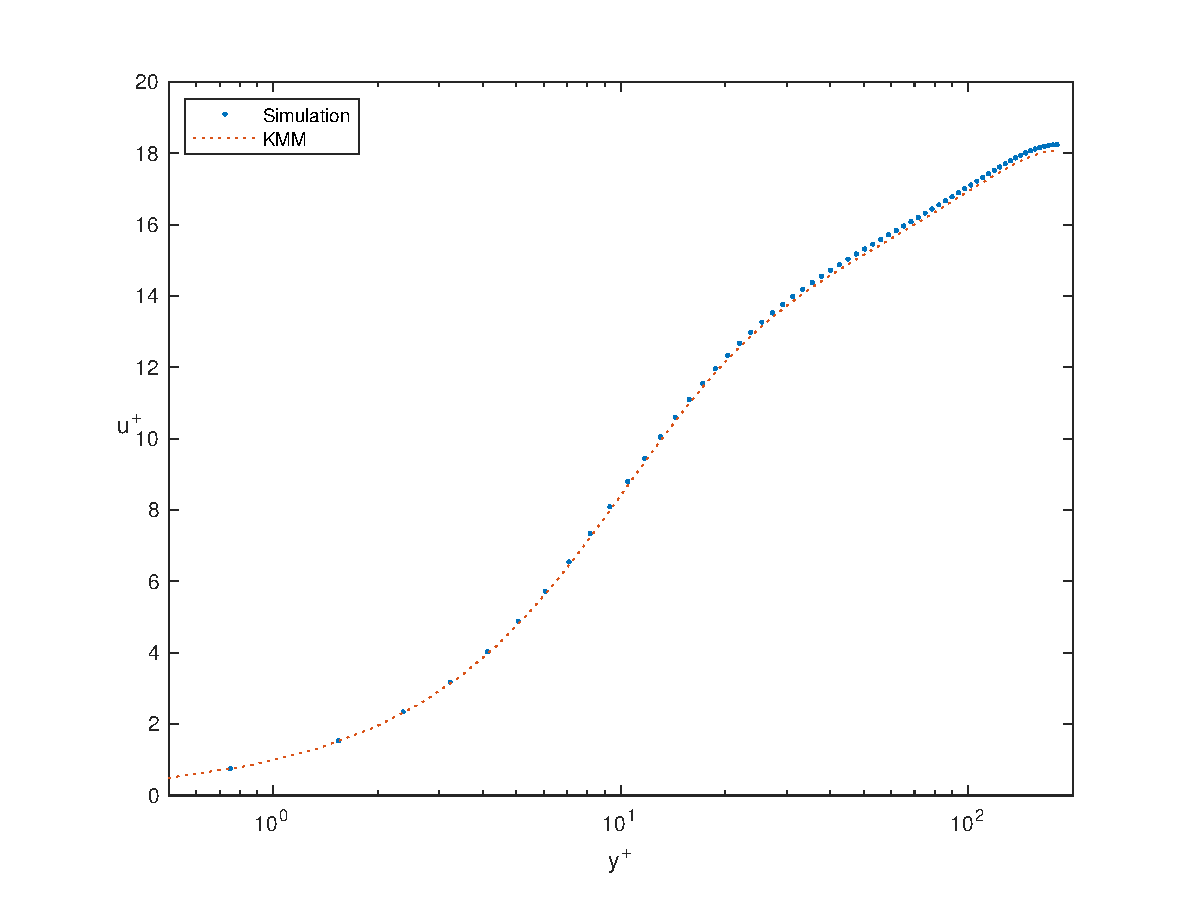
\includegraphics[scale=0.55]{grafici/loglaw_180.eps}
\caption{$\bar{u}^{+}$ in the near wall region for a $Re_{\tau}=180$ simulation}
\label{loglaw_180}
\end{center} 
\end{figure}

\begin{figure}
\begin{center}
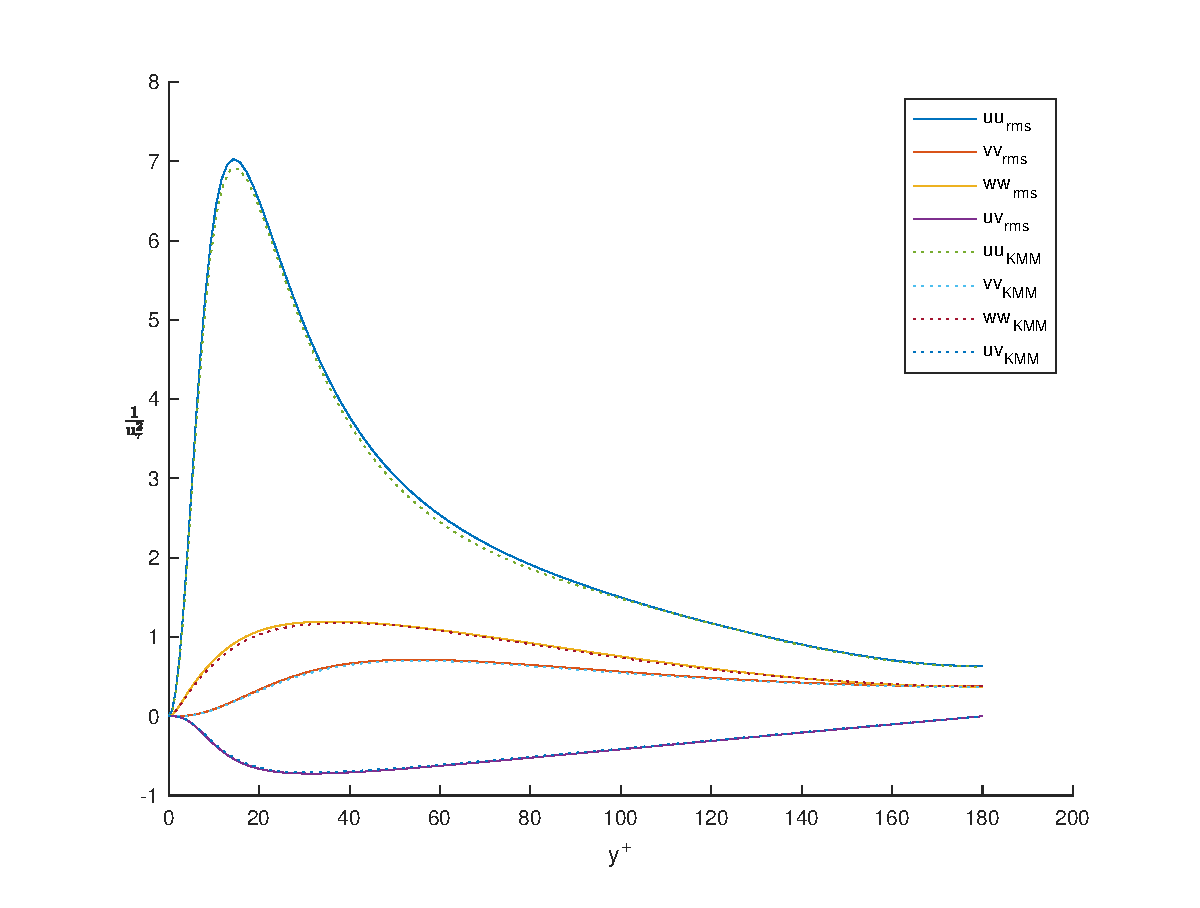
\includegraphics[scale=0.55]{grafici/budget_180.eps}
\caption{TKE budget for a $Re_{\tau}=180$ simulation}
\label{budget_180}
\end{center} 
\end{figure}


Our statistics have been registered using a simulation time of 50 non dimensional units, recording data every 0.1 steps.
In total 500 fields have been used to perform the ensemble average. \par

The data fitting is good, despite being perfect. The differences are related to the fluctuations present in the~\cite{kim_moin_moser} database, which, although well established, is far from being perfect. \\~\par

The results are in agreement with the typical curves behavior, in particular, by looking at the budget curves, we can distinguish the classical peaks, facing $ww^{+} \approx 1.3$ near $y^{+} \approx 35$  ... \par
The figure~\ref{loglaw_180} report the $\bar{u}^{+}$ behavior near the wall. From 0 up to 5 $y^{+}$ units we can see the typical $\bar{u}^{+}=y^{+}$ behavior, which characterize the viscous sublayer. Once $y^{+}>30$ we see the arise of the logarithmic law of the wall, characterized by the equation

\begin{equation*}
\bar{u}^{+} = \frac{1}{\kappa} \ln y^{+} +C^{+},
\end{equation*}

where the Von Karman constant $\kappa=0.41$ and $C^{+}\approx 5.0$, like smooth wall experiments evidenced.
\section{$Re_{\tau}=1000$ simulation} 
The second simulation performed is carried out at $Re_{\tau}=1000$, which in terms of channel width and bulk velocity is equivalent to $Re_{b}\approx40000$.\par
The bulk velocity, obtained as shown in~\ref{bulk:velocity}, is 19.99, while $\alpha_{0}$ and $\beta_{0}$ are respectively 0.5 and 1, in order to reproduce the correct dimensions of the channel, as shown in chapter~\ref{chapter:Re180}.\par
Since the high computational cost needed to obtain these results we were unable to carry out a complete simulation. Thus the results reported show the statistics associated with a flow in a transitory state. \\~\par

The simulation employed a variable timestep, determined through the Courant-Friedrichs-Lewy condition. Since its high computational cost, due to the needed transpositions and Fourier transformations, we decided to set the CFL limit below the stability threshold and calculate it once every $n$ steps. In this way the gain in terms of performance is significant, combining the flexibility of the Courant-Friedrichs-Lewy condition with a reduced cost to compute it.\\~\par

The grid employed in this simulation face 500 points in the wall-normal direction, 2048 in the spanwise direction and 2048 points along the streamwise dimension, direction in which we exploit the Hermitian symmetry. According to this configuration, the grid size reach the billion of points.\par
Table~\ref{table:1000} report a summary of the simulation configuration for the $Re_{\tau}=1000$ case.\\~\par

\begin{table}
\caption{Simulation data for $Re_{\tau}$=1000}
\begin{center}
\begin{tabular}{ccccccccccccc}
\toprule
$L_{x}$ & $L_{z}$ & $\delta$ & $nx$ & $nz$ & $ny$ & $\alpha_{0}$ & $\beta_{0}$ & $\Delta x^{+}$ & $\Delta z^{+}$ & $px$ & $CFL$\\
$4\pi$ & $2\pi$ & 1 & 2048 & 2048 & 500 & 0.5 & 1 & 6.1  & 3 & 1 & 1.6 \\
\bottomrule
\end{tabular}
\end{center}
\label{table:1000}
\end{table}


Since are required approximately 50GB of disk space per each field we decided to avoid to save them on disk, instead we calculated the statistics runtime, merging the files at the end of the simulation, reducing the required space to few KB.\\~\par

The results that we will present shortly are obtained through the ensemble average of 100 fields, and cover 0.1 non dimensional time units. In this lapse of time the mean $Re_{\tau}$ is approximately 991 units and it is slowly moving towards the nominal value of the simulation.\par
Let us focus now on the statistics gained from the simulation.\\~\par
Figure~\ref{loglaw:1000} report the law of the wall. As we can see from the plot, made in semi-logarithmic scale using the wall units, our data fits the theoretical curve throughout the logarithmic region, while, towards the centerline, a residual sensitivity to the initial conditions is still present and lead to few differences with the results obtained by Moser \& Lee in~\cite{Lee}.\par
Far from the wall, the velocity defect law shows acceptable agreement with our results, as figure~\ref{velocity:defect:1000} exhibit.\\~\par

\begin{figure}
\begin{center}
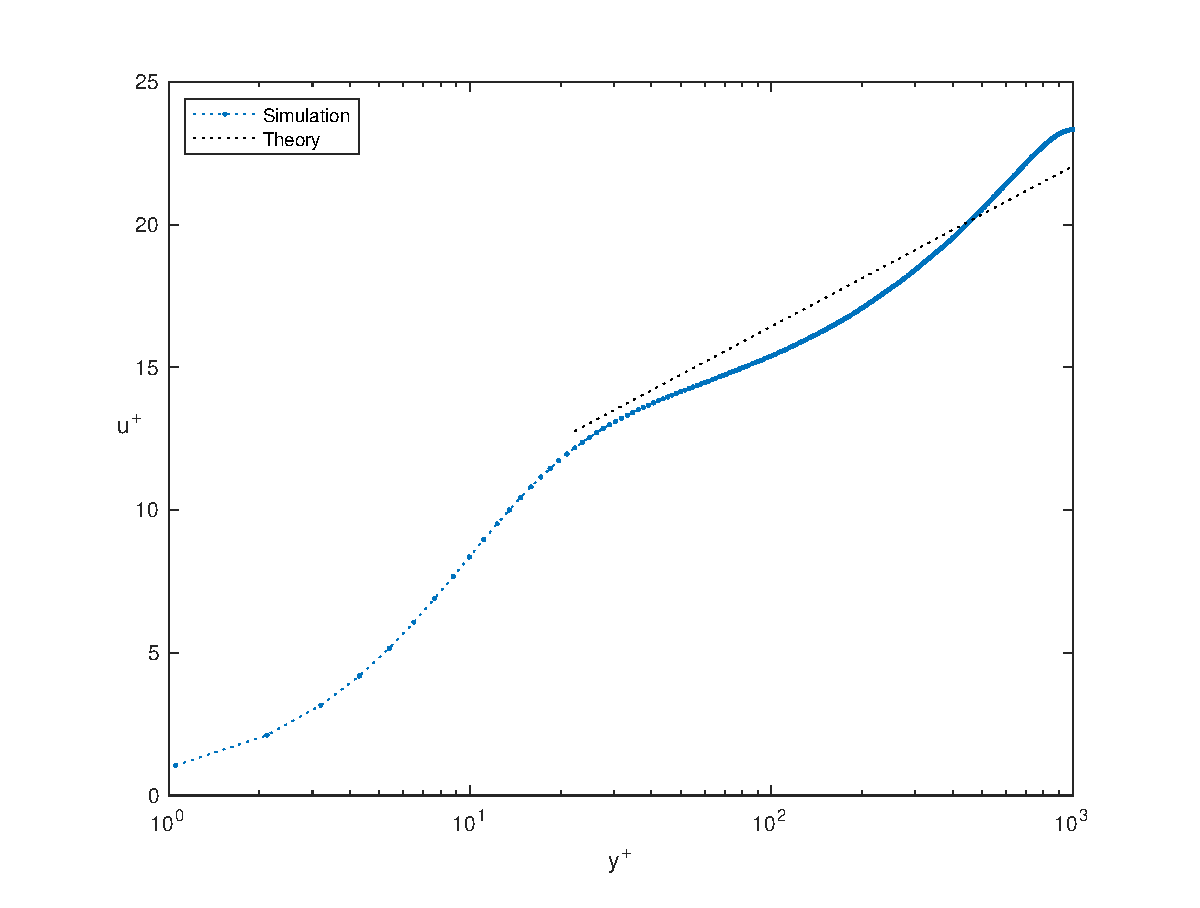
\includegraphics[scale=0.55]{grafici/loglaw_1000.eps}
\caption{$\bar{u}^{+}$ in the near wall region for a $Re_{\tau}=1000$ simulation}
\label{loglaw:1000}
\end{center} 
\end{figure}

\begin{figure}
\begin{center}
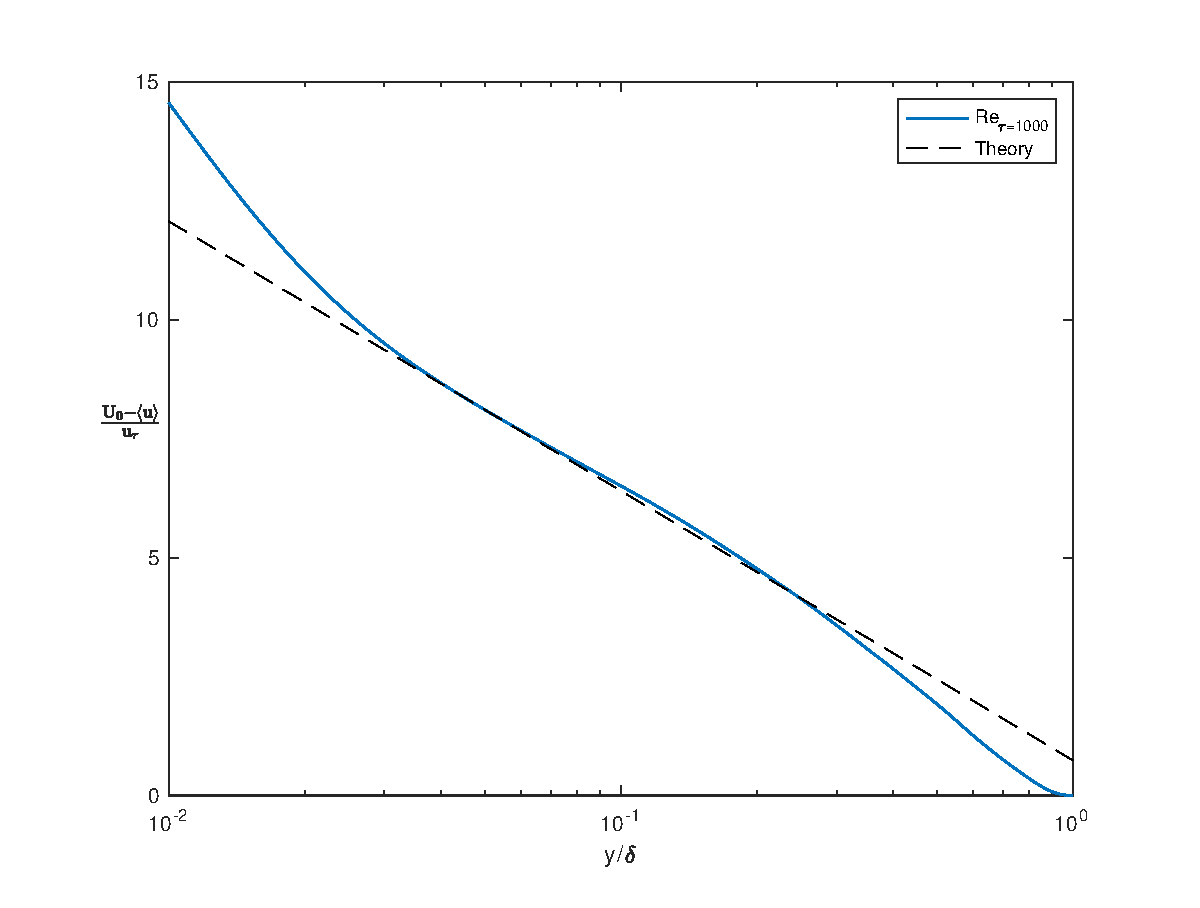
\includegraphics[scale=0.55]{grafici/velocity_defect_1000.eps}
\caption{Velocity defect for a $Re_{\tau}=1000$ simulation}
\label{velocity:defect:1000}
\end{center} 
\end{figure}

In figure~\ref{budget:1000} we reported the \emph{rms} fluctuations, normalized by the $u_{\tau}^{2}$, jointed with the TKE distribution. The first differences that we can immediately face by comparing our curves with the ones in figure~\ref{k+budgets:180} are the peak values. These values tends to increase with respect to the counterpart of the $Re_{\tau}=180$ simulation, highlighting how this simulation contains more energy than the previous ones.\par
Although there is an higher content of energy, the curves shape remains aligned with the ones seen in the previous chapter.\par
The near-wall behavior present a two-components turbulent flow. In fact, as evidenced by the magnification, the wall-normal fluctuations are absent for the first few units.
\\~\par

\begin{figure}
\begin{center}
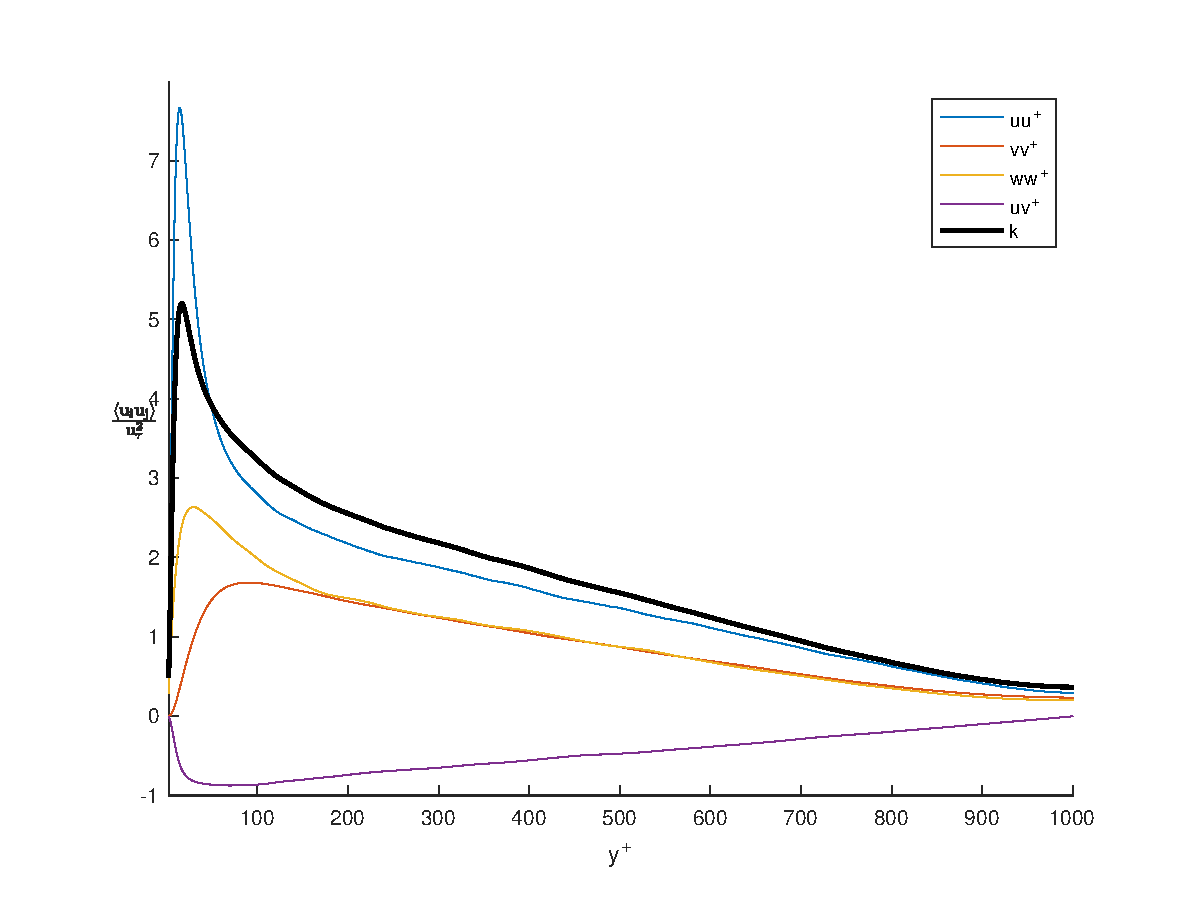
\includegraphics[scale=0.55]{grafici/budget+k_1000.eps}
\caption{\emph{rms} terms for a $Re_{\tau}=1000$ simulation}
\label{budget:1000}
\end{center} 
\end{figure}


The finer mesh and the higher Reynolds evidenced the appearance of a new turbulence peak, detached from the wall-cycle, identified through knees in the curves of figure~\ref{rms:1000}. \par
In such figure our results are compared with the ones of Moser \& Lee, which are the expected values for a complete $Re_{\tau}=1000$ simulation. \par
The results shows accordance among the expected values and the ones obtained through the simulation.
The $u'/u_{\tau}$ curve fits well the expect value, despite the little $Re_{\tau}$ difference among the two datasets.
The $v'/u_{\tau}$ and $w'/u_{\tau}$ curves are in good accordance with the values of Moser \& Lee in the inner region, while towards the centerline of the channel flow we face the raise of differences, possibly due to the transitory nature of the simulation and the dependency on the initial conditions.\\~\par

\begin{figure}
\begin{center}
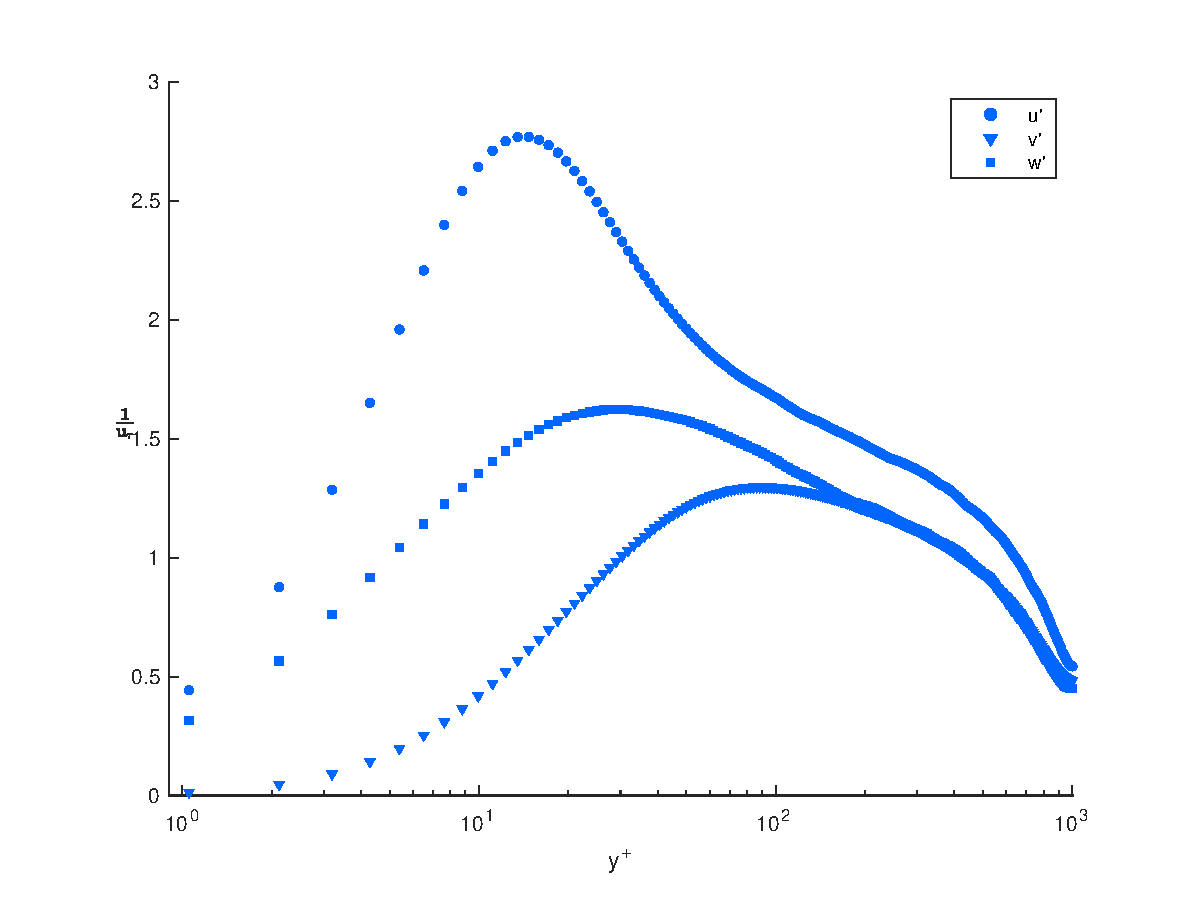
\includegraphics[scale=0.55]{grafici/rms_1000.eps}
\caption{\emph{rms} behavior on a $Re_{\tau}=1000$ simulation}
\label{rms:1000}
\end{center} 
\end{figure}

Comparing the results of this simulation with the ones of the $Re_{\tau}=180$ we can clearly see a generalized upward shift of the \emph{rms} fluctuations. Such trend is present also near the wall. Indeed the curves does not exhibit marked changes in shape with respect to their counterpart in the previous simulation, as figure~\ref{wall:rms:1000} testify, just an upward shift, with the streamwise and spanwise components that depart from zero as $y^{+}$, while the wall-normal components leave the wall as $y^{2+}$. \\~\par

Similar reasoning applies also for the graphs of the \emph{production}, reported in figure~\ref{tke:prod:1000}, that reach a slightly higher peak of $P/Re_{\tau}=0.24$, without showing significant changes of the curve shape. The peak is still located nearby $y\approx 12$.\\~\par

As theory affirms, the wall coordinate of the peak of production corresponds to that in which the stress components become equivalent. This aspect will be investigated further, comparing the results of the two simulations together.
At the present time we limit to illustrate the behavior of the stress components, which are reported in figure~\ref{stresses:1000}. As we can see, the normalized total shear stress is quasi-straight, suggesting that we are still in a transitory phase. The driving-train of this unsteadiness has to be searched in the excess of Reynolds stresses, which are forcing our flow towards higher Reynolds values. \par
\begin{figure}
\begin{center}
\includegraphics[scale=0.55]{grafici/wall_rms_1000.eps}
\caption{Normalized \emph{rms} close to the wall for a $Re_{\tau}=1000$ simulation}
\label{wall:rms:1000}
\end{center} 
\end{figure}

\begin{figure}
\begin{center}
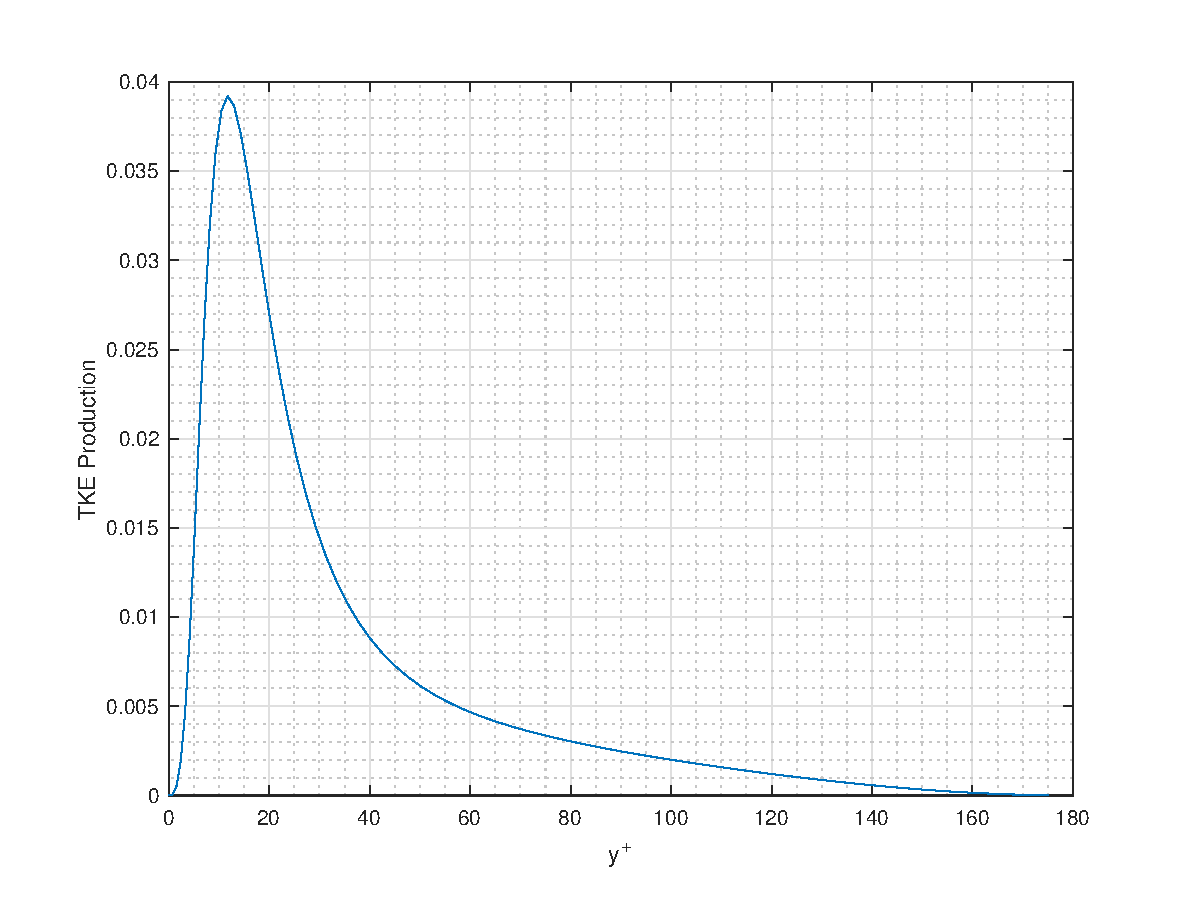
\includegraphics[scale=0.55]{grafici/tke_prod_1000.eps}
\caption{Production term of the TKE eq. for a $Re_{\tau}=1000$ simulation}
\label{tke:prod:1000}
\end{center} 
\end{figure}

\begin{figure}
\begin{center}
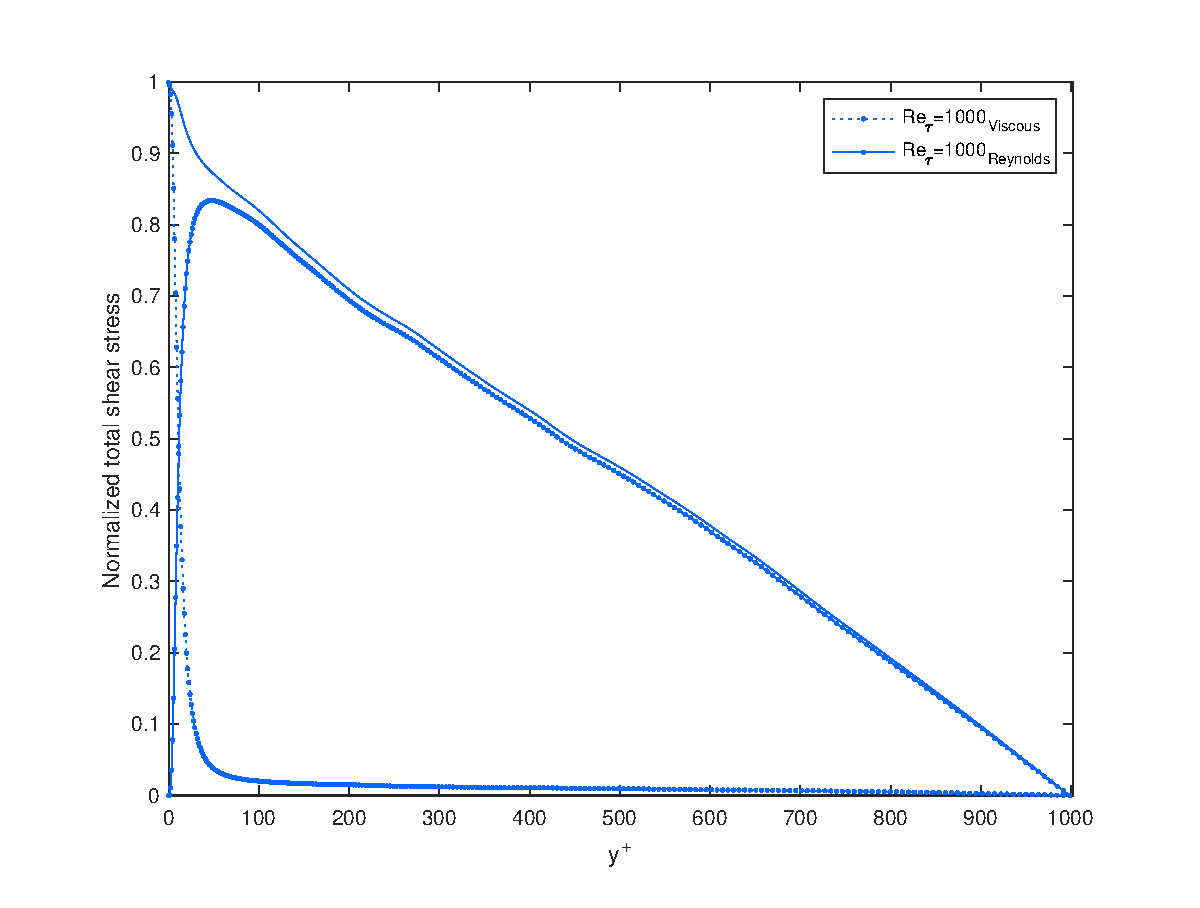
\includegraphics[scale=0.55]{grafici/stresses_1000.eps}
\caption{Normalized total shear stress for a $Re_{\tau}=1000$ simulation}
\label{stresses:1000}
\end{center} 
\end{figure}
%\section{$Re_{\tau}=2000$ simulation} 
The last simulation performed is carried out at $Re_{\tau}\approx2000$, which in terms of channel width and bulk velocity is approximately equivalent to $Re_{b}=100000$.\par
The bulk velocity is 24.3, $\alpha_{0}$ is 0.5 and $\beta_{0}$ is equal to 1.\par
The timestep is constant, with \emph{dt}=0.00001 and the simulation time is T=1. \par
The excessive resource requests lead us to perform a reduced simulation, able just to highlight the principal features of this $Re_{\tau}$. The simulation time, indeed, is reduced to a single non-dimensional units, however, in order to guarantee good results, we sampled the field every 0.001 steps, so that we can employ a 1000 fields to do the ensemble average.\\~\par
The grid employed in this simulation face 1000 points in the wall-normal direction, 4096 in the spanwise direction and 4096 points along the streamwise dimension. The mesh size is extremely huge, with more than 8 billions of points.\par
We reported a summary of the simulation configuration in table~\ref{table:2000}\\~\par

\begin{table}
\caption{Simulation data for $Re_{\tau}$=2000}
\begin{center}
\begin{tabular}{ccccccccccccc}
\toprule
$L_{x}$ & $L_{z}$ & $\delta$ & $nx$ & $nz$ & $ny$ & $\alpha_{0}$ & $\beta_{0}$ & $\Delta x^{+}$ & $\Delta z^{+}$ & $px$ & $dt$ & $T$\\
$4\pi$ & $2\pi$ & 1 & 4096 & 4096 & 1000 & 0.5 & 1 & 6.1  & 3 & 1 & 0.00002 & 1 \\
\bottomrule
\end{tabular}
\end{center}
\label{table:2000}
\end{table}


The disk space requirement raised approximately by a factor of 10, with 400GB of disk space needed per each field. This reason pushed us once again to rely in live post processing, instead of saving snapshots of the field.\\~\par

The statistics gained from the simulation are here presented.\par
We start from figure~\ref{loglaw:2000}, which report the law of the wall. Despite the graph is not perfect, during the simulation the data has shown a tendency to re-align with the theoretical behavior, characterized by $k=0.41$ and $B=5.2$. As consequence, towards the centerline, the velocity defect law is affected by fluctuations caused by the poor temporal resolution, as shown by the graph~\ref{velocity:defect:2000}. Despite these fluctuations, it is possible to see that the region subject to linearity has grown again \\~\par

\begin{figure}
\begin{center}
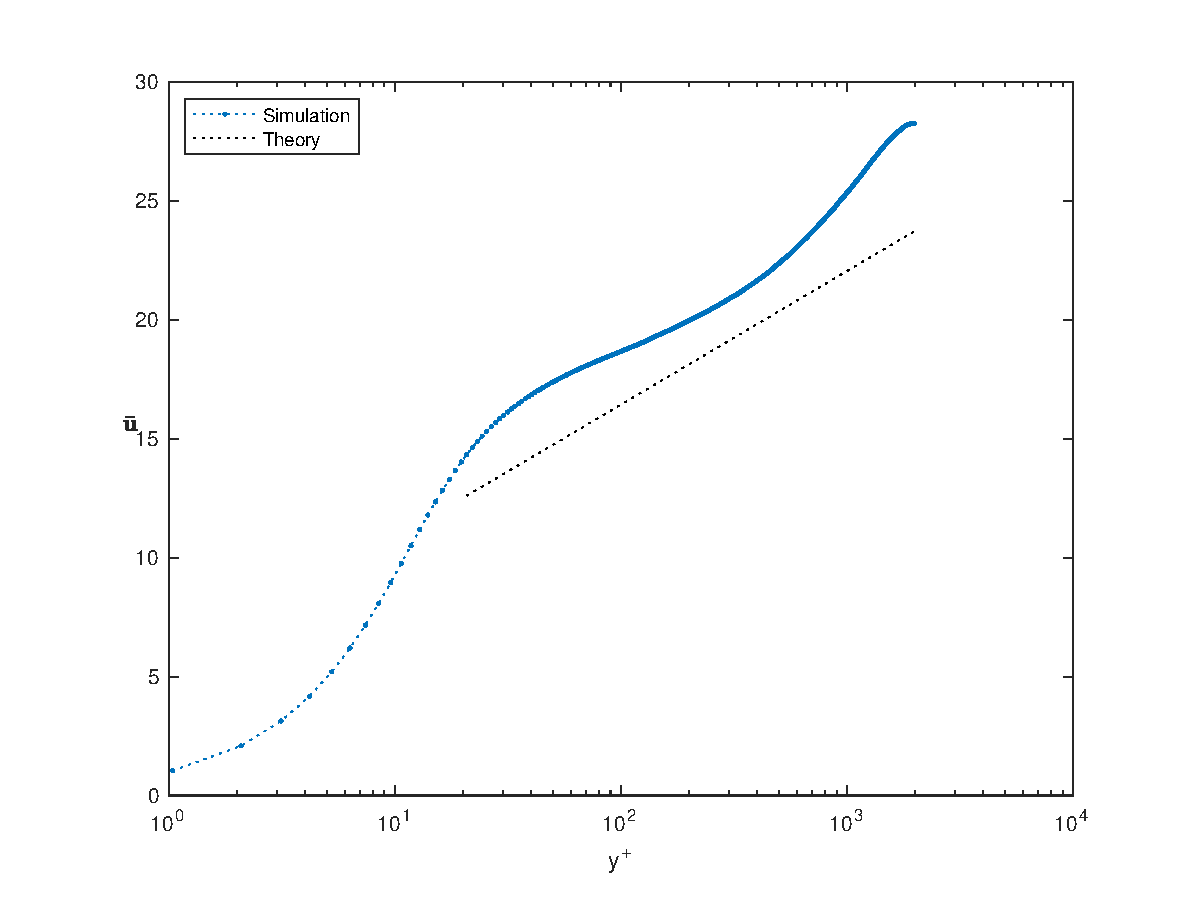
\includegraphics[scale=0.55]{grafici/loglaw_2000.eps}
\caption{$\bar{u}^{+}$ in the near wall region for a $Re_{\tau}=2000$ simulation}
\label{loglaw:2000}
\end{center} 
\end{figure}

\begin{figure}
\begin{center}
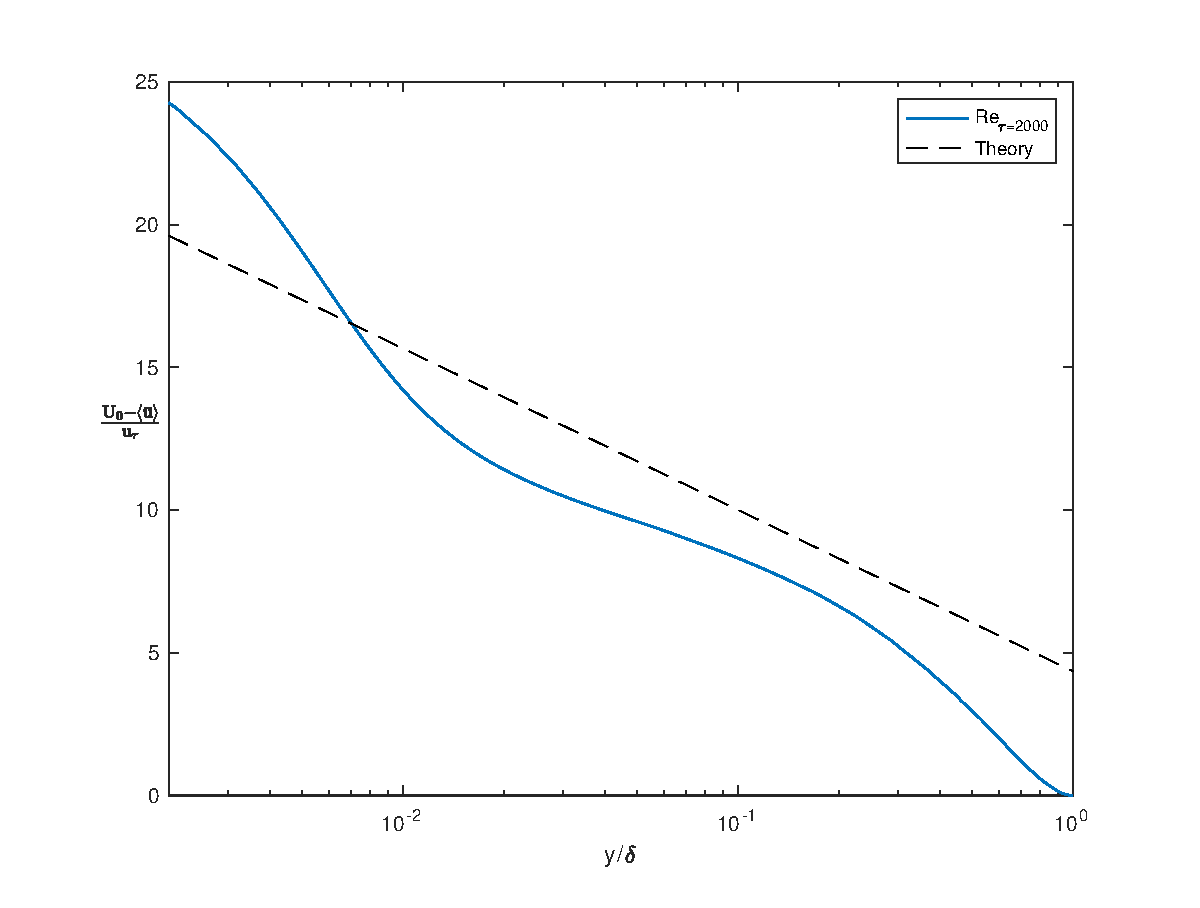
\includegraphics[scale=0.55]{grafici/velocity_defect_2000.eps}
\caption{Velocity defect for a $Re_{\tau}=2000$ simulation}
\label{velocity:defect:2000}
\end{center} 
\end{figure}

In figure~\ref{budget:2000} we reported the \emph{rms} fluctuations, normalized by the $u_{\tau}^{2}$, jointed with the TKE distribution. The first difference we can see by comparing this graph with the others is related to the peak values, which have incremented again, in line with our expectations for a more turbulent flow. \par
This time we can see that, followed by the raise in peak values, the spanwise and streamwise fluctuations exhibit a wider basement, with more energy   associated to those distances from the wall. This fact is partially due to the reduced lengthscale of this simulation with respect to the previous.\par
However, as the lens magnify, despite of the higher $Re_{\tau}$, the turbulence still tend to exhibit itself as a bi-dimensional phenomena close to the wall, exactly what happens also for \emph{low Reynolds} simulations.\par

Reaching the centerline the \emph{rms} terms and the TKE curve tends to align with the values of the $Re_{\tau}=1000$ simulation.\\~\par

\begin{figure}
\begin{center}
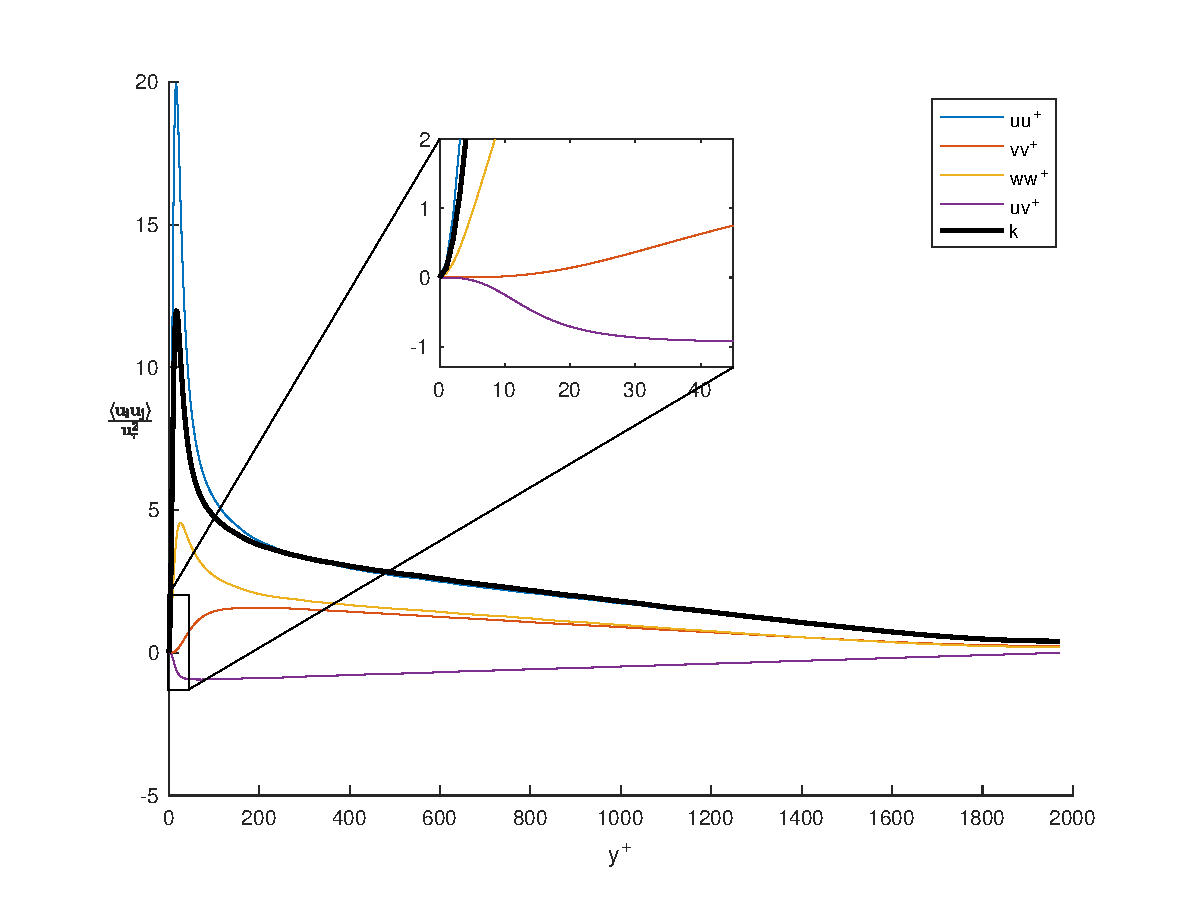
\includegraphics[scale=0.55]{grafici/budget+k_2000.eps}
\caption{\emph{rms} terms for a $Re_{\tau}=2000$ simulation}
\label{budget:2000}
\end{center} 
\end{figure}


The raise in Reynolds number modified the fluctuations distribution with a generalized upward shift, as figure~\ref{rms:2000} report, pushing the peaks towards higher values, with the peaks coordinate remaining approximately constant. The knee tends to move rightward for all the \emph{rms} terms, towards the centerline. Also the outer-cycle peaks tend to exhibit an upward shift, however it results to be lower than the previous boost.\\~\par

\begin{figure}
\begin{center}
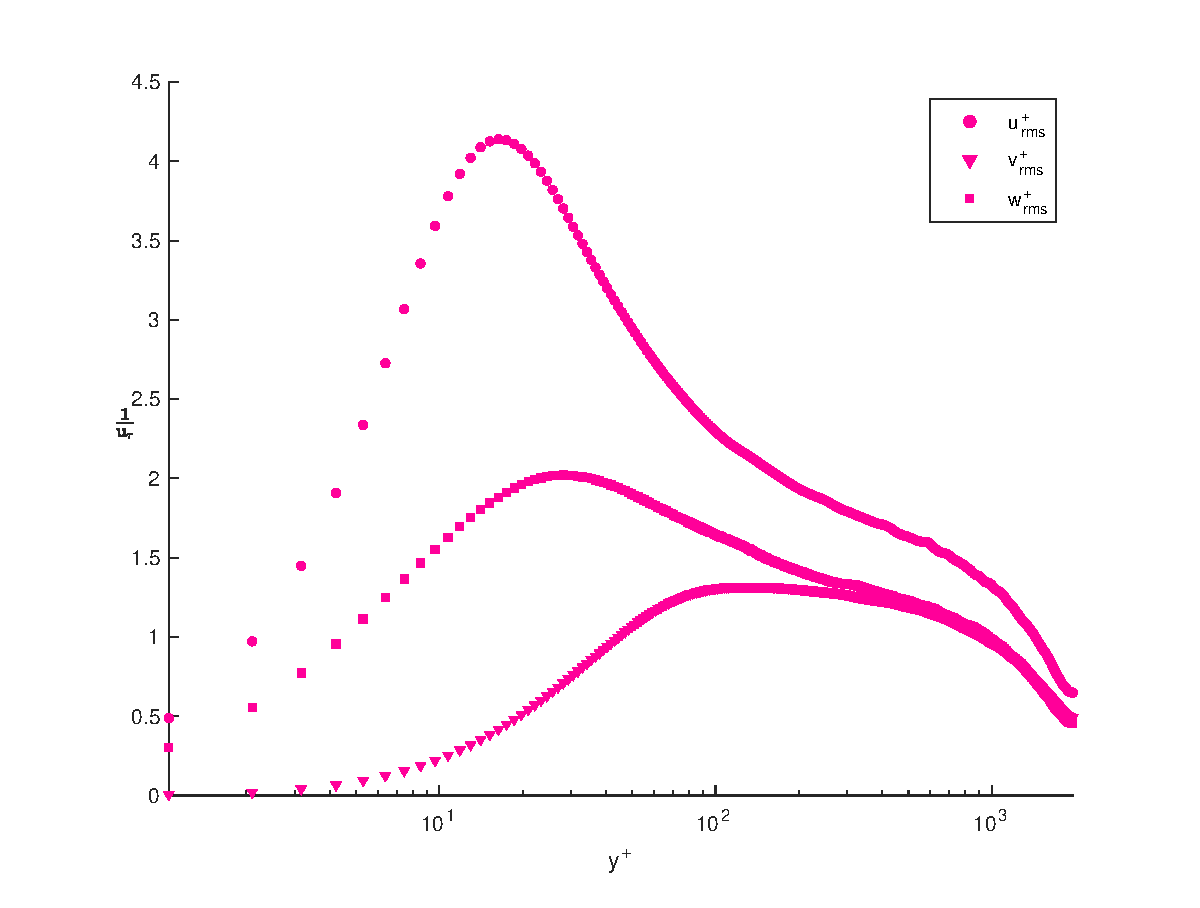
\includegraphics[scale=0.55]{grafici/rms_2000.eps}
\caption{\emph{rms} behavior on a $Re_{\tau}=2000$ simulation}
\label{rms:2000}
\end{center} 
\end{figure}

\begin{figure}
\begin{center}
\includegraphics[scale=0.55]{grafici/wall_rms_2000.eps}
\caption{Normalized \emph{rms} close to the wall for a $Re_{\tau}=2000$ simulation}
\label{wall:rms:2000}
\end{center} 
\end{figure}

The streamwise and spanwise \emph{rms} terms tends to be higher since they leave the wall, this can be caught by comparing figure~\ref{wall:rms:2000} with figure~\ref{wall:rms:1000}. As can be recovered from the plot, such curves exhibit a linear growth for a wider range of wall coordinates, with respect to previous simulations. \par
The wall-normal fluctuation develops perfectly as $y^{+2}$ and its starting value is lower than the ones in previous simulations.\\~\par


For what concern about the \emph{production} term of the turbulent kinetic energy, according to figure~\ref{tke:prod:2000}, we can see that there are no changes to the profile, with the peak which remains near $y\approx12$. \\~\par

The normalized total shear stress profile is presented in figure~\ref{stresses:2000}. The graph exhibit the typical profile, with the Reynolds stresses that grows immediately and reach their peak before $y^{+}\approx 100$. \par
The crossing point between the viscous stress and Reynolds ones is still around $y\approx12$. This will be shown in the next chapter with an higher level of detail.


\begin{figure}
\begin{center}
\includegraphics[scale=0.55]{grafici/tke_prod_2000.eps}
\caption{Production term of the TKE eq. for a $Re_{\tau}=2000$ simulation}
\label{tke:prod:2000}
\end{center} 
\end{figure}

\begin{figure}
\begin{center}
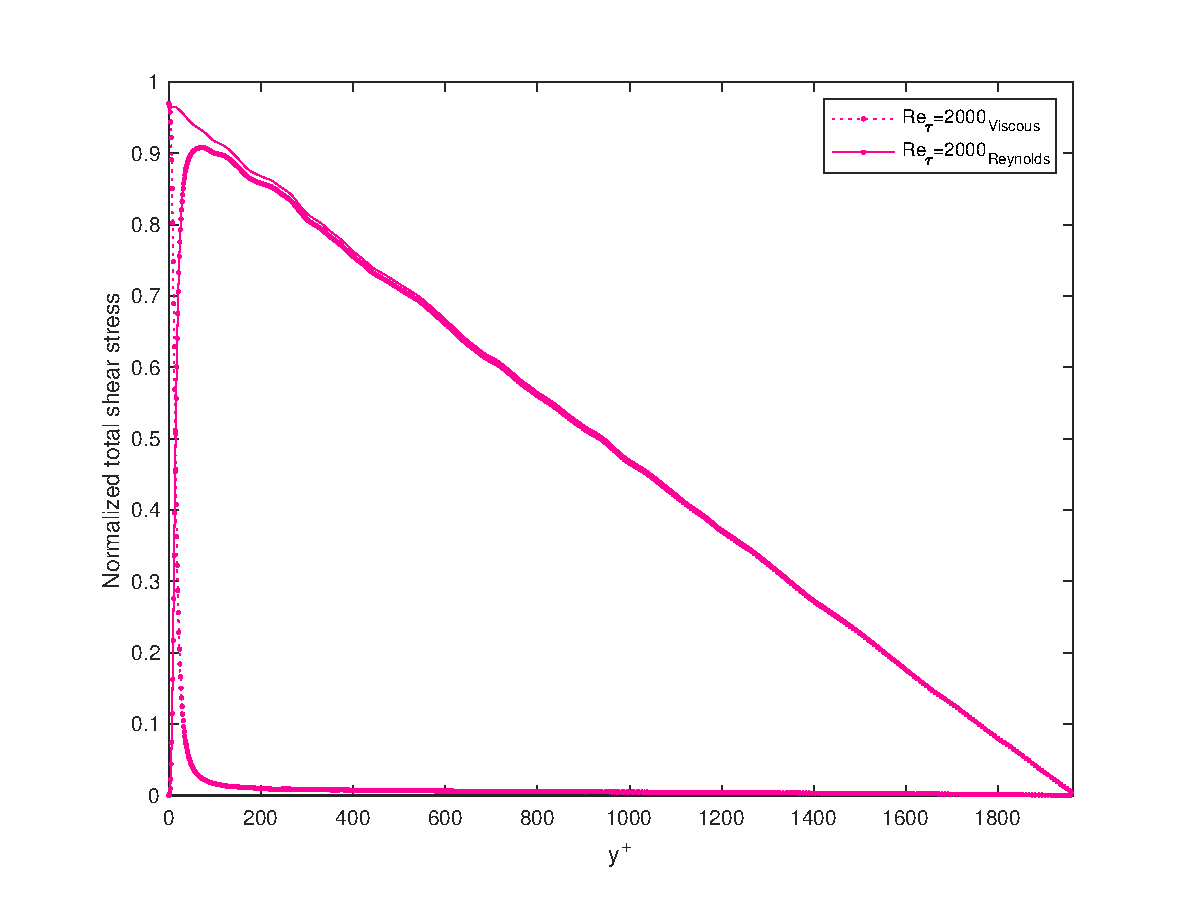
\includegraphics[scale=0.55]{grafici/stresses_2000.eps}
\caption{Normalized total shear stress for a $Re_{\tau}=2000$ simulation}
\label{stresses:2000}
\end{center} 
\end{figure}
\section{Reynolds effects}
We are now interested to catch the effects of the Reynolds on our statistics.\\~\par
The firstly macroscopical effect that we face is a shift, towards higher values, of the mean velocity profile. The shadowed area of figure~\ref{mean:comparison} let us enjoy the previous statement. According to this graph we can see a progressive narrowing of the region subjected to the higher shear stress, as the Reynolds number becomes larger.\par
Under the previous graph we reported the same quantity, but presented in semi-logaritmic scale, using both inner and outer scaling.
The first plot of figure~\ref{loglaw:comparison} highlights the results of the simulations and the theoretical behavior expectations.
In particular we can see that, despite the Reynolds number, all the simulations present the linear $\bar{u}=y^{+}$ behavior expected in the viscous sublayer, and the logarithmic profile in the homonym region, with $k=0.41$ and $B=5.2$.\\~\par

\begin{figure}
\begin{center}
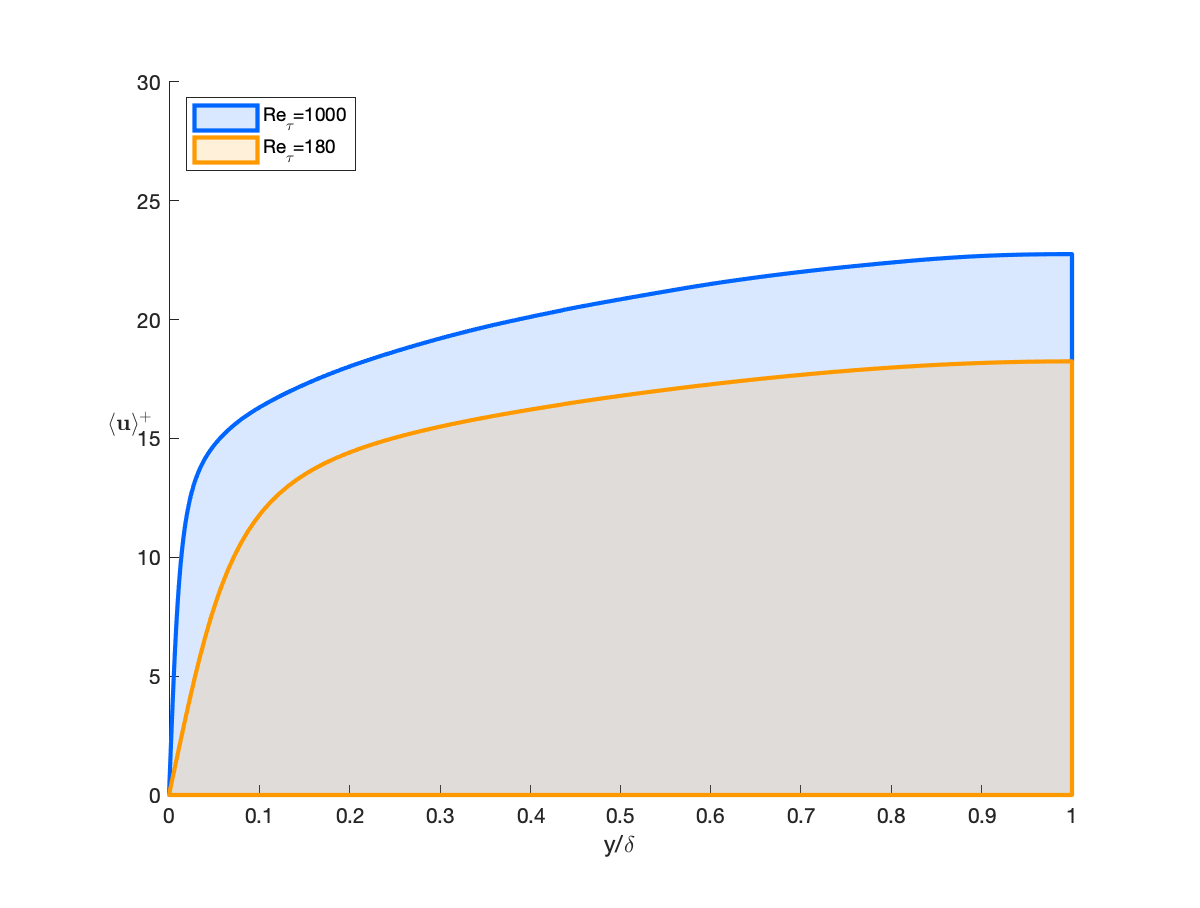
\includegraphics[scale=0.55]{grafici/u_mean_comparison.eps}
\caption{Mean velocity profile at $Re_{\tau}$ variation}
\label{mean:comparison}
\end{center}
\end{figure}
\begin{figure}
\begin{center}
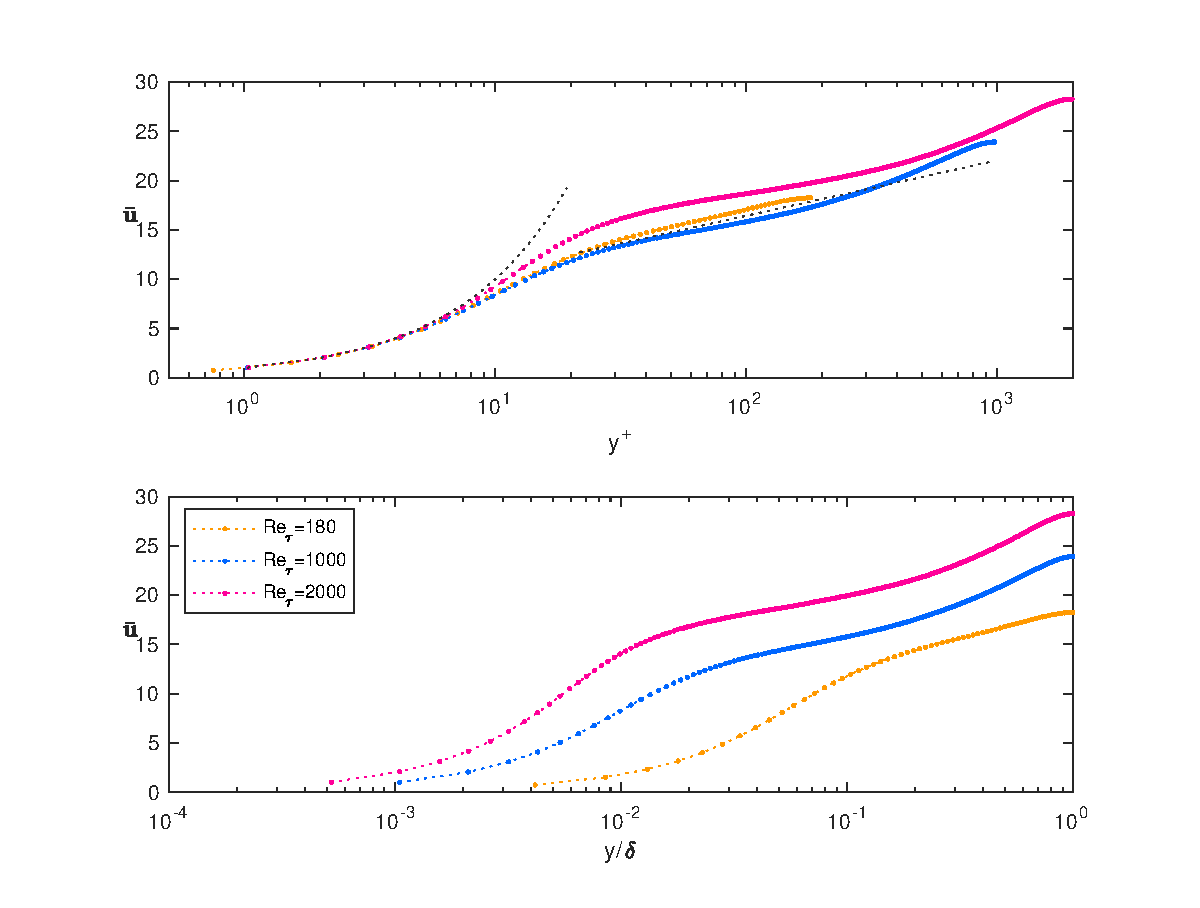
\includegraphics[scale=0.55]{grafici/loglaw_comparison.eps}
\caption{The law of the wall, in inner and outer scaling, at $Re_{\tau}$ variation}
\label{loglaw:comparison}
\end{center}
\end{figure}


Differently, the Reynolds stresses and the viscous stress exhibit dependance on the Reynolds number.\par
Figure~\ref{shear:comparison} shows how the shear stress components modify as the Reynolds number increase. \par
Focusing on the normalized Reynolds stresses graph we can clearly see that, as the $Re_{\tau}$ increase, the region subjected to this kind of stresses becomes larger, with the peak moving towards the wall. Such kind of stress is associated with the fluid turbulent motions, therefore it was expectable a raise of this components as we move towards a more turbulent flow. \par

\begin{figure}
\begin{center}
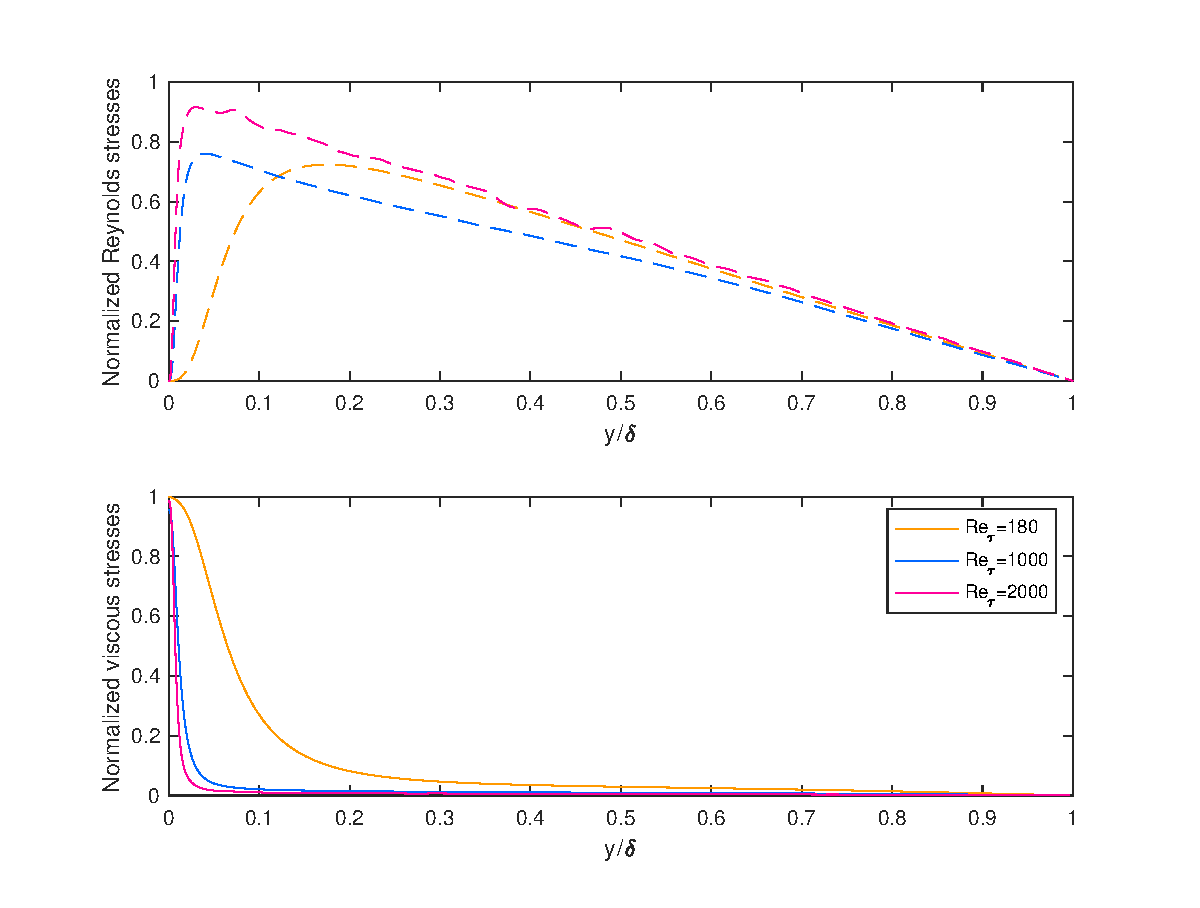
\includegraphics[scale=0.55]{grafici/shear_comparison.eps}
\caption{Normalized shear profiles at $Re_{\tau}$ variation}
\label{shear:comparison}
\end{center}
\end{figure}

\begin{figure}
\begin{center}
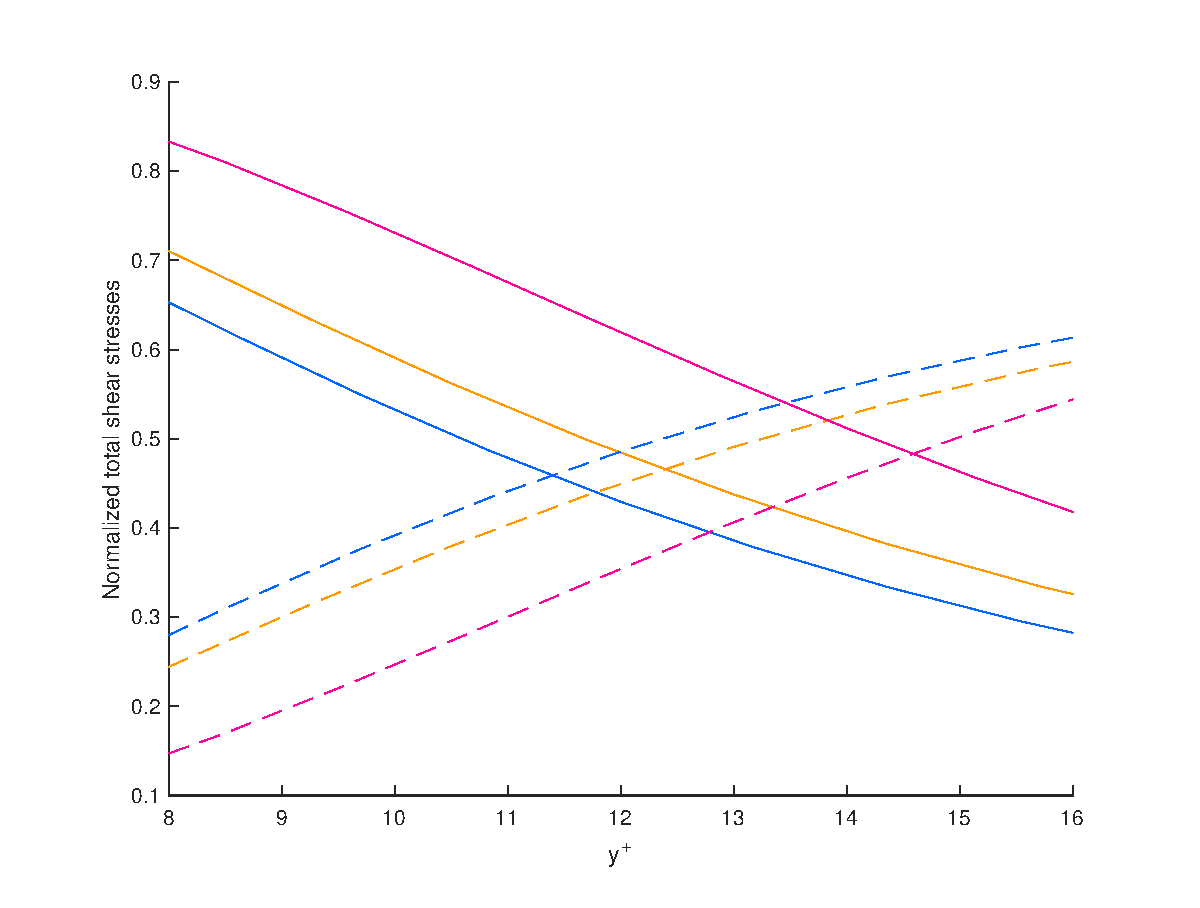
\includegraphics[scale=0.55]{grafici/y12.eps}
\caption{Particular of the shear stress, at $Re_{\tau}$ variation}
\label{y12}
\end{center}
\end{figure}

On the other side the contribute of the viscous stress, associate to $\partial{\bar{u}}/\partial{t}$, is maximum at the wall and tends to become negligible as we move towards the centerline. \par
As testified by figure~\ref{loglaw:comparison}, the higher is the Reynolds and the wider is the area subjected to logarithmic profile, hence smaller is the area subjected to strong variation of the mean velocity profile with the wall-normal coordinate. This fact reflects on our shear component reducing its range of effectiveness to few units, close to the wall, as the $Re$ grows.\par
Although, in terms of outer scaling, the stress components are subjected to strong variations, in inner scaling we can see, in figure~\ref{y12}, that the point at which the two components cross themself remains quite constant, with an $y^{+}$ around 12 wall-units.\\~\par


\begin{figure}
\begin{center}
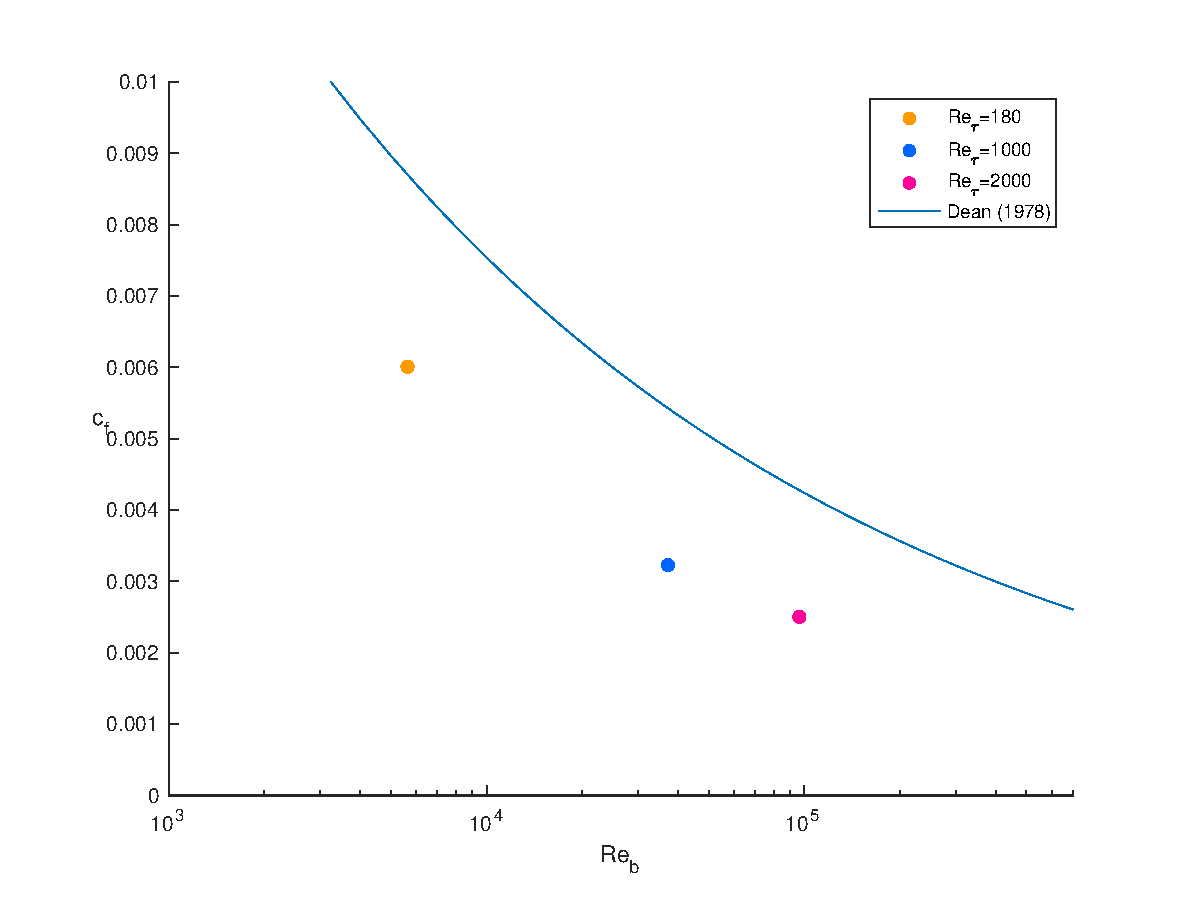
\includegraphics[scale=0.55]{grafici/cf.eps}
\caption{Dependance of the $c_{f}$ from $Re_{b}$}
\label{cf}
\end{center}
\end{figure}


One of the most important flow property for wall bounded flows is the friction coefficient.
The $c_{f}$ has been studied in detail by many famous authors of the past: Nikuradse, Prandtl, Blasius just to cite some of them. \par
In our simulations we computed the skin friction coefficient based on the definition provided by~\cite[279]{pope}, based on centerline velocity $(U_{0})$ and the $Re_{b}$ of the channel.
The quantities have been defined as
\begin{equation*}
c_{f}= 2(\frac{u_{\tau}}{U_{0}})^{2}	\quad~\quad~\quad~\quad	Re_{b}= \frac{2 U_{b} \delta}{\nu},
\end{equation*}
and the results have been reported on figure~\ref{cf}. \par
Our $c_{f}$ shows good fitting with the results of the experimental campaign of Dean reported in~\cite{Dean}.



\chapter{Conclusions \& Further Works}

I am glad to say that we have reached our original goal to provide a scalable DNS solver through the usage of the MPI technology. \par
At present time the code lacks in an intra-nodal effectively parallelization, therefore its performances are limited by the MPI local communication performance. Despite of this the code revealed to be robust, being capable of working both with small datasets then extra large ones, exhibiting a linear gain in terms of productivity.
The possibility to perform live post-processing of the data, instead of writing them, allows to save terabytes of memory, allowing the code to run also on networks of commodity hardware. \\~\par
The fundamental restriction imposed by the original code about the number of parallel tasks has been removed, bringing the theoretical number of parallel processes to be limited by the product of $nx \times nz$ modes. \\~\par
The engine developed is flexible and since is not affected by the geometry of the problem could be adapted quickly to carry out boundary layers simulations, just by imposing different boundary conditions, or can be used to solve pipe flows simulations.\\~\par

The intent of this work was just to provide a study of feasibility for a solver based on pencil decomposition approach relying on inter-nodal parallelization, therefore we are satisfied by the results obtained. It should be denoted that, at present time, we cannot consider this as a ``completed'' solver. The lack of a dedicated shared memory parallelization reduce the efficiency significantly. However, we would like to highlight that a dedicated shared memory parallelization could be carried out just by changing few rows, without the needing of a significant reworking of the code.
With today tendency of the HPC processors to increase the number of threads, instead of the number of physical CPU, this evolution, towards the so called \emph{hybrid-programming}, seems mandatory.


\backmatter
\addcontentsline{toc}{chapter}{\bibname} 
\printbibliography

\end{document}
